\documentclass[12pt,twoside]{article}
% =====================================================================
%  preambulo.tex
%  Paquetes, configuración de página y estilo para bloques de código.
%  Se carga desde main.tex con % =====================================================================
%  preambulo.tex
%  Paquetes, configuración de página y estilo para bloques de código.
%  Se carga desde main.tex con % =====================================================================
%  preambulo.tex
%  Paquetes, configuración de página y estilo para bloques de código.
%  Se carga desde main.tex con \input{preambulo}
% =====================================================================

% ---------------------------------------------------------------------
%  Codificación, idioma y fuentes
% ---------------------------------------------------------------------
\usepackage[T1]{fontenc}          % acentos y guiones correctos en español
\usepackage[utf8]{inputenc}
\usepackage{lmodern}              % versión vectorial de Computer Modern
\usepackage[spanish,es-tabla]{babel}
\usepackage{titlesec}

% ---------------------------------------------------------------------
%  Geometría de página y encabezados
% ---------------------------------------------------------------------
\usepackage[a4paper, width=150mm, top=25mm, bottom=25mm, bindingoffset=6mm]{geometry}
\usepackage{fancyhdr}
\setlength{\headheight}{15.4pt}   % evita el warning de fancyhdr
\pagestyle{fancy}
\fancyhead{}
\fancyhead[LO,LE]{\leftmark}
\fancyfoot{}
\fancyfoot[CO,CE]{\thepage}
\renewcommand{\headrulewidth}{0.2pt}
\renewcommand{\footrulewidth}{0.2pt}

% ---------------------------------------------------------------------
%  Colores (antes que otros paquetes que puedan cargarlo)
% ---------------------------------------------------------------------
\usepackage[dvipsnames,table]{xcolor}
% Color para los diagramas TikZ (verde esmeralda)
\definecolor{emerald}{RGB}{5,150,105}

% ---------------------------------------------------------------------
%  Matemáticas y símbolos
% ---------------------------------------------------------------------
\usepackage{amsmath}
\numberwithin{table}{section}
\numberwithin{figure}{section}
\numberwithin{equation}{section} % ecuaciones: (capítulo.número)
\usepackage{amssymb}
\usepackage{textcomp}
\usepackage{siunitx}

% ---------------------------------------------------------------------
%  Tablas
% ---------------------------------------------------------------------
\usepackage{array}
\usepackage{longtable}
\usepackage{multirow}
\usepackage{bigstrut}
\usepackage{booktabs}
\usepackage{tabularx}

% ---------------------------------------------------------------------
%  Figuras y páginas horizontales
% ---------------------------------------------------------------------
\usepackage{graphicx}
\usepackage{adjustbox}
\usepackage{float}
\usepackage{lscape}
\usepackage{pdflscape}
\usepackage{subcaption}
% Separador entre el número y el texto del caption: "Tabla 2.3. Descripción"
\captionsetup{labelsep=period}

% ---------------------------------------------------------------------
%  Diagramas con TikZ
% ---------------------------------------------------------------------
\usepackage{tikz}
\usetikzlibrary{shapes.geometric, arrows.meta, positioning, fit, backgrounds, calc, shadows}
\usetikzlibrary{babel} % evita conflictos de TikZ con los caracteres activos de babel en español

% ---------------------------------------------------------------------
%  Bibliografía (formato IEEE: citas numéricas entre corchetes)
% ---------------------------------------------------------------------
\usepackage{notoccite}
\usepackage[numbers, sort&compress]{natbib}
\usepackage[nottoc]{tocbibind}

% ---------------------------------------------------------------------
%  Apéndices
% ---------------------------------------------------------------------
\usepackage[toc,page]{appendix}

% ---------------------------------------------------------------------
%  Código fuente: paquete listings + estilo "codigo"
% ---------------------------------------------------------------------
\usepackage{listings}

% Paleta inspirada en la imagen de referencia
\definecolor{codFondo}{HTML}{FAFAFB}      % fondo casi blanco
\definecolor{codMarco}{HTML}{D0D0D5}      % borde gris claro
\definecolor{codTexto}{HTML}{2B2B2B}      % variables e identificadores
\definecolor{codPalabra}{HTML}{5B8BC9}    % def, if, else, return...
\definecolor{codFuncion}{HTML}{4A7FC1}    % nombres de funciones (emph)
\definecolor{codNumero}{HTML}{6AA56A}     % números
\definecolor{codComentario}{HTML}{8C8C8C} % comentarios
\definecolor{codCadena}{HTML}{C1693C}     % cadenas de texto
\definecolor{codNumLinea}{HTML}{A0A0A0}   % números de línea

% Colorea los dígitos solo cuando están en código (no en comentarios ni cadenas)
\makeatletter
\newcommand{\codDigito}[1]{%
  \ifnum\lst@mode=\lst@Pmode\relax
    {\color{codNumero}#1}%
  \else
    #1%
  \fi
}
\makeatother

% Mostrar hasta el nivel 4 numerado
\setcounter{secnumdepth}{4}
\setcounter{tocdepth}{4} % el índice muestra hasta el nivel 4 (paragraph)

% Formato de \paragraph en línea nueva
\titleformat{\paragraph}
  {\normalfont\normalsize\bfseries}
  {\theparagraph}{1em}{}
\titlespacing*{\paragraph}{0pt}{3.25ex plus 1ex minus .2ex}{1.5ex plus .2ex}

\lstdefinestyle{codigo}{
  language=Python,
  % --- Tipografía y colores ---
  basicstyle=\ttfamily\small\color{codTexto},
  identifierstyle=\color{codTexto},
  keywordstyle=\color{codPalabra},
  keywordstyle=[2]\color{codPalabra},
  emphstyle=\color{codFuncion},
  commentstyle=\color{codComentario},
  stringstyle=\color{codCadena},
  % --- Palabras reservadas adicionales ---
  morekeywords=[2]{True, False, None, self, nonlocal, async, await},
  % --- Marco y fondo ---
  backgroundcolor=\color{codFondo},
  frame=single,
  frameround=tttt,          % las cuatro esquinas redondeadas
  framerule=0.6pt,
  rulecolor=\color{codMarco},
  framesep=8pt,
  xleftmargin=9pt,
  xrightmargin=9pt,
  aboveskip=1em,
  belowskip=1em,
  % --- Espaciado y cortes de línea ---
  columns=fullflexible,
  keepspaces=true,
  showstringspaces=false,
  tabsize=4,
  breaklines=true,
  breakatwhitespace=true,
  postbreak=\mbox{\textcolor{codComentario}{$\hookrightarrow$}\space},
  upquote=true,
  % --- Números de línea (cambia a "left" si los quieres) ---
  numbers=none,
  numberstyle=\tiny\color{codNumLinea},
  % --- Acentos en español y coloreado de números ---
  extendedchars=true,
  literate=
    {á}{{\'a}}1 {é}{{\'e}}1 {í}{{\'i}}1 {ó}{{\'o}}1 {ú}{{\'u}}1
    {Á}{{\'A}}1 {É}{{\'E}}1 {Í}{{\'I}}1 {Ó}{{\'O}}1 {Ú}{{\'U}}1
    {ñ}{{\~n}}1 {Ñ}{{\~N}}1 {ü}{{\"u}}1 {Ü}{{\"U}}1
    {¿}{{?`}}1 {¡}{{!`}}1
    {0}{{\codDigito{0}}}1 {1}{{\codDigito{1}}}1 {2}{{\codDigito{2}}}1
    {3}{{\codDigito{3}}}1 {4}{{\codDigito{4}}}1 {5}{{\codDigito{5}}}1
    {6}{{\codDigito{6}}}1 {7}{{\codDigito{7}}}1 {8}{{\codDigito{8}}}1
    {9}{{\codDigito{9}}}1
}

% Estilo por defecto para todos los lstlisting
\lstset{style=codigo}

% ---------------------------------------------------------------------
%  Nombres en español
%  1) Se agregan a los nombres que babel activa para el español.
%  2) Se fuerzan otra vez al empezar el documento, para que ningún
%     paquete los regrese al inglés.
% ---------------------------------------------------------------------
\addto\captionsspanish{%
  \def\contentsname{Índice general}%
  \def\listfigurename{Índice de figuras}%
  \def\listtablename{Índice de tablas}%
  \def\tablename{Tabla}%
  \def\refname{Referencias}%
  \def\appendixname{Apéndice}%
  \def\appendixtocname{Apéndices}%
  \def\appendixpagename{Apéndices}%
}

\AtBeginDocument{%
  \renewcommand{\contentsname}{Índice general}%
  \renewcommand{\listfigurename}{Índice de figuras}%
  \renewcommand{\listtablename}{Índice de tablas}%
  \renewcommand{\tablename}{Tabla}%
  \renewcommand{\refname}{Referencias}%
  \renewcommand{\appendixname}{Apéndice}%
  \renewcommand{\appendixtocname}{Apéndices}%
  \renewcommand{\appendixpagename}{Apéndices}%
  \renewcommand{\lstlistingname}{Código}%
  \renewcommand{\lstlistlistingname}{Índice de códigos}%
}

% ---------------------------------------------------------------------
%  Enlaces (hyperref debe ir al final)
% ---------------------------------------------------------------------
\usepackage{url}
\usepackage[hidelinks]{hyperref}

\sloppy
\hyphenpenalty=10000
\exhyphenpenalty=10000

% =====================================================================

% ---------------------------------------------------------------------
%  Codificación, idioma y fuentes
% ---------------------------------------------------------------------
\usepackage[T1]{fontenc}          % acentos y guiones correctos en español
\usepackage[utf8]{inputenc}
\usepackage{lmodern}              % versión vectorial de Computer Modern
\usepackage[spanish,es-tabla]{babel}
\usepackage{titlesec}

% ---------------------------------------------------------------------
%  Geometría de página y encabezados
% ---------------------------------------------------------------------
\usepackage[a4paper, width=150mm, top=25mm, bottom=25mm, bindingoffset=6mm]{geometry}
\usepackage{fancyhdr}
\setlength{\headheight}{15.4pt}   % evita el warning de fancyhdr
\pagestyle{fancy}
\fancyhead{}
\fancyhead[LO,LE]{\leftmark}
\fancyfoot{}
\fancyfoot[CO,CE]{\thepage}
\renewcommand{\headrulewidth}{0.2pt}
\renewcommand{\footrulewidth}{0.2pt}

% ---------------------------------------------------------------------
%  Colores (antes que otros paquetes que puedan cargarlo)
% ---------------------------------------------------------------------
\usepackage[dvipsnames,table]{xcolor}
% Color para los diagramas TikZ (verde esmeralda)
\definecolor{emerald}{RGB}{5,150,105}

% ---------------------------------------------------------------------
%  Matemáticas y símbolos
% ---------------------------------------------------------------------
\usepackage{amsmath}
\numberwithin{table}{section}
\numberwithin{figure}{section}
\numberwithin{equation}{section} % ecuaciones: (capítulo.número)
\usepackage{amssymb}
\usepackage{textcomp}
\usepackage{siunitx}

% ---------------------------------------------------------------------
%  Tablas
% ---------------------------------------------------------------------
\usepackage{array}
\usepackage{longtable}
\usepackage{multirow}
\usepackage{bigstrut}
\usepackage{booktabs}
\usepackage{tabularx}

% ---------------------------------------------------------------------
%  Figuras y páginas horizontales
% ---------------------------------------------------------------------
\usepackage{graphicx}
\usepackage{adjustbox}
\usepackage{float}
\usepackage{lscape}
\usepackage{pdflscape}
\usepackage{subcaption}
% Separador entre el número y el texto del caption: "Tabla 2.3. Descripción"
\captionsetup{labelsep=period}

% ---------------------------------------------------------------------
%  Diagramas con TikZ
% ---------------------------------------------------------------------
\usepackage{tikz}
\usetikzlibrary{shapes.geometric, arrows.meta, positioning, fit, backgrounds, calc, shadows}
\usetikzlibrary{babel} % evita conflictos de TikZ con los caracteres activos de babel en español

% ---------------------------------------------------------------------
%  Bibliografía (formato IEEE: citas numéricas entre corchetes)
% ---------------------------------------------------------------------
\usepackage{notoccite}
\usepackage[numbers, sort&compress]{natbib}
\usepackage[nottoc]{tocbibind}

% ---------------------------------------------------------------------
%  Apéndices
% ---------------------------------------------------------------------
\usepackage[toc,page]{appendix}

% ---------------------------------------------------------------------
%  Código fuente: paquete listings + estilo "codigo"
% ---------------------------------------------------------------------
\usepackage{listings}

% Paleta inspirada en la imagen de referencia
\definecolor{codFondo}{HTML}{FAFAFB}      % fondo casi blanco
\definecolor{codMarco}{HTML}{D0D0D5}      % borde gris claro
\definecolor{codTexto}{HTML}{2B2B2B}      % variables e identificadores
\definecolor{codPalabra}{HTML}{5B8BC9}    % def, if, else, return...
\definecolor{codFuncion}{HTML}{4A7FC1}    % nombres de funciones (emph)
\definecolor{codNumero}{HTML}{6AA56A}     % números
\definecolor{codComentario}{HTML}{8C8C8C} % comentarios
\definecolor{codCadena}{HTML}{C1693C}     % cadenas de texto
\definecolor{codNumLinea}{HTML}{A0A0A0}   % números de línea

% Colorea los dígitos solo cuando están en código (no en comentarios ni cadenas)
\makeatletter
\newcommand{\codDigito}[1]{%
  \ifnum\lst@mode=\lst@Pmode\relax
    {\color{codNumero}#1}%
  \else
    #1%
  \fi
}
\makeatother

% Mostrar hasta el nivel 4 numerado
\setcounter{secnumdepth}{4}
\setcounter{tocdepth}{4} % el índice muestra hasta el nivel 4 (paragraph)

% Formato de \paragraph en línea nueva
\titleformat{\paragraph}
  {\normalfont\normalsize\bfseries}
  {\theparagraph}{1em}{}
\titlespacing*{\paragraph}{0pt}{3.25ex plus 1ex minus .2ex}{1.5ex plus .2ex}

\lstdefinestyle{codigo}{
  language=Python,
  % --- Tipografía y colores ---
  basicstyle=\ttfamily\small\color{codTexto},
  identifierstyle=\color{codTexto},
  keywordstyle=\color{codPalabra},
  keywordstyle=[2]\color{codPalabra},
  emphstyle=\color{codFuncion},
  commentstyle=\color{codComentario},
  stringstyle=\color{codCadena},
  % --- Palabras reservadas adicionales ---
  morekeywords=[2]{True, False, None, self, nonlocal, async, await},
  % --- Marco y fondo ---
  backgroundcolor=\color{codFondo},
  frame=single,
  frameround=tttt,          % las cuatro esquinas redondeadas
  framerule=0.6pt,
  rulecolor=\color{codMarco},
  framesep=8pt,
  xleftmargin=9pt,
  xrightmargin=9pt,
  aboveskip=1em,
  belowskip=1em,
  % --- Espaciado y cortes de línea ---
  columns=fullflexible,
  keepspaces=true,
  showstringspaces=false,
  tabsize=4,
  breaklines=true,
  breakatwhitespace=true,
  postbreak=\mbox{\textcolor{codComentario}{$\hookrightarrow$}\space},
  upquote=true,
  % --- Números de línea (cambia a "left" si los quieres) ---
  numbers=none,
  numberstyle=\tiny\color{codNumLinea},
  % --- Acentos en español y coloreado de números ---
  extendedchars=true,
  literate=
    {á}{{\'a}}1 {é}{{\'e}}1 {í}{{\'i}}1 {ó}{{\'o}}1 {ú}{{\'u}}1
    {Á}{{\'A}}1 {É}{{\'E}}1 {Í}{{\'I}}1 {Ó}{{\'O}}1 {Ú}{{\'U}}1
    {ñ}{{\~n}}1 {Ñ}{{\~N}}1 {ü}{{\"u}}1 {Ü}{{\"U}}1
    {¿}{{?`}}1 {¡}{{!`}}1
    {0}{{\codDigito{0}}}1 {1}{{\codDigito{1}}}1 {2}{{\codDigito{2}}}1
    {3}{{\codDigito{3}}}1 {4}{{\codDigito{4}}}1 {5}{{\codDigito{5}}}1
    {6}{{\codDigito{6}}}1 {7}{{\codDigito{7}}}1 {8}{{\codDigito{8}}}1
    {9}{{\codDigito{9}}}1
}

% Estilo por defecto para todos los lstlisting
\lstset{style=codigo}

% ---------------------------------------------------------------------
%  Nombres en español
%  1) Se agregan a los nombres que babel activa para el español.
%  2) Se fuerzan otra vez al empezar el documento, para que ningún
%     paquete los regrese al inglés.
% ---------------------------------------------------------------------
\addto\captionsspanish{%
  \def\contentsname{Índice general}%
  \def\listfigurename{Índice de figuras}%
  \def\listtablename{Índice de tablas}%
  \def\tablename{Tabla}%
  \def\refname{Referencias}%
  \def\appendixname{Apéndice}%
  \def\appendixtocname{Apéndices}%
  \def\appendixpagename{Apéndices}%
}

\AtBeginDocument{%
  \renewcommand{\contentsname}{Índice general}%
  \renewcommand{\listfigurename}{Índice de figuras}%
  \renewcommand{\listtablename}{Índice de tablas}%
  \renewcommand{\tablename}{Tabla}%
  \renewcommand{\refname}{Referencias}%
  \renewcommand{\appendixname}{Apéndice}%
  \renewcommand{\appendixtocname}{Apéndices}%
  \renewcommand{\appendixpagename}{Apéndices}%
  \renewcommand{\lstlistingname}{Código}%
  \renewcommand{\lstlistlistingname}{Índice de códigos}%
}

% ---------------------------------------------------------------------
%  Enlaces (hyperref debe ir al final)
% ---------------------------------------------------------------------
\usepackage{url}
\usepackage[hidelinks]{hyperref}

\sloppy
\hyphenpenalty=10000
\exhyphenpenalty=10000

% =====================================================================

% ---------------------------------------------------------------------
%  Codificación, idioma y fuentes
% ---------------------------------------------------------------------
\usepackage[T1]{fontenc}          % acentos y guiones correctos en español
\usepackage[utf8]{inputenc}
\usepackage{lmodern}              % versión vectorial de Computer Modern
\usepackage[spanish,es-tabla]{babel}
\usepackage{titlesec}

% ---------------------------------------------------------------------
%  Geometría de página y encabezados
% ---------------------------------------------------------------------
\usepackage[a4paper, width=150mm, top=25mm, bottom=25mm, bindingoffset=6mm]{geometry}
\usepackage{fancyhdr}
\setlength{\headheight}{15.4pt}   % evita el warning de fancyhdr
\pagestyle{fancy}
\fancyhead{}
\fancyhead[LO,LE]{\leftmark}
\fancyfoot{}
\fancyfoot[CO,CE]{\thepage}
\renewcommand{\headrulewidth}{0.2pt}
\renewcommand{\footrulewidth}{0.2pt}

% ---------------------------------------------------------------------
%  Colores (antes que otros paquetes que puedan cargarlo)
% ---------------------------------------------------------------------
\usepackage[dvipsnames,table]{xcolor}
% Color para los diagramas TikZ (verde esmeralda)
\definecolor{emerald}{RGB}{5,150,105}

% ---------------------------------------------------------------------
%  Matemáticas y símbolos
% ---------------------------------------------------------------------
\usepackage{amsmath}
\numberwithin{table}{section}
\numberwithin{figure}{section}
\numberwithin{equation}{section} % ecuaciones: (capítulo.número)
\usepackage{amssymb}
\usepackage{textcomp}
\usepackage{siunitx}

% ---------------------------------------------------------------------
%  Tablas
% ---------------------------------------------------------------------
\usepackage{array}
\usepackage{longtable}
\usepackage{multirow}
\usepackage{bigstrut}
\usepackage{booktabs}
\usepackage{tabularx}

% ---------------------------------------------------------------------
%  Figuras y páginas horizontales
% ---------------------------------------------------------------------
\usepackage{graphicx}
\usepackage{adjustbox}
\usepackage{float}
\usepackage{lscape}
\usepackage{pdflscape}
\usepackage{subcaption}
% Separador entre el número y el texto del caption: "Tabla 2.3. Descripción"
\captionsetup{labelsep=period}

% ---------------------------------------------------------------------
%  Diagramas con TikZ
% ---------------------------------------------------------------------
\usepackage{tikz}
\usetikzlibrary{shapes.geometric, arrows.meta, positioning, fit, backgrounds, calc, shadows}
\usetikzlibrary{babel} % evita conflictos de TikZ con los caracteres activos de babel en español

% ---------------------------------------------------------------------
%  Bibliografía (formato IEEE: citas numéricas entre corchetes)
% ---------------------------------------------------------------------
\usepackage{notoccite}
\usepackage[numbers, sort&compress]{natbib}
\usepackage[nottoc]{tocbibind}

% ---------------------------------------------------------------------
%  Apéndices
% ---------------------------------------------------------------------
\usepackage[toc,page]{appendix}

% ---------------------------------------------------------------------
%  Código fuente: paquete listings + estilo "codigo"
% ---------------------------------------------------------------------
\usepackage{listings}

% Paleta inspirada en la imagen de referencia
\definecolor{codFondo}{HTML}{FAFAFB}      % fondo casi blanco
\definecolor{codMarco}{HTML}{D0D0D5}      % borde gris claro
\definecolor{codTexto}{HTML}{2B2B2B}      % variables e identificadores
\definecolor{codPalabra}{HTML}{5B8BC9}    % def, if, else, return...
\definecolor{codFuncion}{HTML}{4A7FC1}    % nombres de funciones (emph)
\definecolor{codNumero}{HTML}{6AA56A}     % números
\definecolor{codComentario}{HTML}{8C8C8C} % comentarios
\definecolor{codCadena}{HTML}{C1693C}     % cadenas de texto
\definecolor{codNumLinea}{HTML}{A0A0A0}   % números de línea

% Colorea los dígitos solo cuando están en código (no en comentarios ni cadenas)
\makeatletter
\newcommand{\codDigito}[1]{%
  \ifnum\lst@mode=\lst@Pmode\relax
    {\color{codNumero}#1}%
  \else
    #1%
  \fi
}
\makeatother

% Mostrar hasta el nivel 4 numerado
\setcounter{secnumdepth}{4}
\setcounter{tocdepth}{4} % el índice muestra hasta el nivel 4 (paragraph)

% Formato de \paragraph en línea nueva
\titleformat{\paragraph}
  {\normalfont\normalsize\bfseries}
  {\theparagraph}{1em}{}
\titlespacing*{\paragraph}{0pt}{3.25ex plus 1ex minus .2ex}{1.5ex plus .2ex}

\lstdefinestyle{codigo}{
  language=Python,
  % --- Tipografía y colores ---
  basicstyle=\ttfamily\small\color{codTexto},
  identifierstyle=\color{codTexto},
  keywordstyle=\color{codPalabra},
  keywordstyle=[2]\color{codPalabra},
  emphstyle=\color{codFuncion},
  commentstyle=\color{codComentario},
  stringstyle=\color{codCadena},
  % --- Palabras reservadas adicionales ---
  morekeywords=[2]{True, False, None, self, nonlocal, async, await},
  % --- Marco y fondo ---
  backgroundcolor=\color{codFondo},
  frame=single,
  frameround=tttt,          % las cuatro esquinas redondeadas
  framerule=0.6pt,
  rulecolor=\color{codMarco},
  framesep=8pt,
  xleftmargin=9pt,
  xrightmargin=9pt,
  aboveskip=1em,
  belowskip=1em,
  % --- Espaciado y cortes de línea ---
  columns=fullflexible,
  keepspaces=true,
  showstringspaces=false,
  tabsize=4,
  breaklines=true,
  breakatwhitespace=true,
  postbreak=\mbox{\textcolor{codComentario}{$\hookrightarrow$}\space},
  upquote=true,
  % --- Números de línea (cambia a "left" si los quieres) ---
  numbers=none,
  numberstyle=\tiny\color{codNumLinea},
  % --- Acentos en español y coloreado de números ---
  extendedchars=true,
  literate=
    {á}{{\'a}}1 {é}{{\'e}}1 {í}{{\'i}}1 {ó}{{\'o}}1 {ú}{{\'u}}1
    {Á}{{\'A}}1 {É}{{\'E}}1 {Í}{{\'I}}1 {Ó}{{\'O}}1 {Ú}{{\'U}}1
    {ñ}{{\~n}}1 {Ñ}{{\~N}}1 {ü}{{\"u}}1 {Ü}{{\"U}}1
    {¿}{{?`}}1 {¡}{{!`}}1
    {0}{{\codDigito{0}}}1 {1}{{\codDigito{1}}}1 {2}{{\codDigito{2}}}1
    {3}{{\codDigito{3}}}1 {4}{{\codDigito{4}}}1 {5}{{\codDigito{5}}}1
    {6}{{\codDigito{6}}}1 {7}{{\codDigito{7}}}1 {8}{{\codDigito{8}}}1
    {9}{{\codDigito{9}}}1
}

% Estilo por defecto para todos los lstlisting
\lstset{style=codigo}

% ---------------------------------------------------------------------
%  Nombres en español
%  1) Se agregan a los nombres que babel activa para el español.
%  2) Se fuerzan otra vez al empezar el documento, para que ningún
%     paquete los regrese al inglés.
% ---------------------------------------------------------------------
\addto\captionsspanish{%
  \def\contentsname{Índice general}%
  \def\listfigurename{Índice de figuras}%
  \def\listtablename{Índice de tablas}%
  \def\tablename{Tabla}%
  \def\refname{Referencias}%
  \def\appendixname{Apéndice}%
  \def\appendixtocname{Apéndices}%
  \def\appendixpagename{Apéndices}%
}

\AtBeginDocument{%
  \renewcommand{\contentsname}{Índice general}%
  \renewcommand{\listfigurename}{Índice de figuras}%
  \renewcommand{\listtablename}{Índice de tablas}%
  \renewcommand{\tablename}{Tabla}%
  \renewcommand{\refname}{Referencias}%
  \renewcommand{\appendixname}{Apéndice}%
  \renewcommand{\appendixtocname}{Apéndices}%
  \renewcommand{\appendixpagename}{Apéndices}%
  \renewcommand{\lstlistingname}{Código}%
  \renewcommand{\lstlistlistingname}{Índice de códigos}%
}

% ---------------------------------------------------------------------
%  Enlaces (hyperref debe ir al final)
% ---------------------------------------------------------------------
\usepackage{url}
\usepackage[hidelinks]{hyperref}

\sloppy
\hyphenpenalty=10000
\exhyphenpenalty=10000
 % paquetes, formato de página y estilo de código

\begin{document}
\bibliographystyle{achemso} % estilo de citas, cámbialo si es necesario

\begin{titlepage}
\begin{center}
         
\includegraphics[width=15cm]{logos} %this is to have the logo
         \vspace{3cm}
         
        \Large
        \textbf{TRADUCCIÓN AUTOMÁTICA DE TEXTO A PICTOGRAMAS MEDIANTE MODELOS TRANSFORMER}\\
        \vspace{0.5cm}
        \large
       Trabajo Terminal No. 2027-A036 %of X
     
        \vspace{1.5cm}
     \large
        \textbf{Robles Guzmán Naomi Isabel,\\ Ugalde Téllez Aarón} %add any letters that should follow like B.Sc. or M.Sc. or AMRSC etc
        
        \vfill
        
        \normalsize
        \textbf{como requisito para el título de Ingeniería en Inteligencia Artificial} 
            
        \vfill
            
        \large 
        \textbf{Directores: }Winfield Reyes Ana María, Vásquez Gómez Juan Irving
            
        \vfill
            
        \large
        Escuela Superior de Cómputo\\
        Instituto Politécnico Nacional $-$ IPN\\
        Ciudad de México, México\\
        Noviembre, 2026
            
    \end{center}

\end{titlepage}
 % portada

\tableofcontents % índice general (el título en español se define en preambulo.tex)

%\include{Thanks-abstact} % Resumen y agradecimientos

% Capítulos: usa \include{archivo} para cada .tex
\pagenumbering{arabic} %necessary to start numbering pages in arabic numerals from here
\setcounter{page}{1} 

\section{Introducción}
\subsection{Problemática}
La comunicación es un derecho humano fundamental. Sin embargo, personas con discapacidades del lenguaje enfrentan barreras significativas para expresarse. La Comunicación Aumentativa y Alternativa (CAA) ofrece una solución mediante el uso de pictogramas, los cuales son representaciones visuales de conceptos que permiten transmitir mensajes sin depender del lenguaje verbal convencional \cite{beukelman2013}.

El Portal Aragonés de Comunicación Aumentativa y Alternativa (ARASAAC) es uno de los sistemas pictográficos más utilizados a nivel mundial, con más de 12,000 pictogramas de uso libre \cite{arasaac2007}. A pesar de la disponibilidad de estos recursos, la traducción automática de lenguaje natural a secuencias de pictogramas sigue siendo un reto.

Para ilustrar la complejidad del problema, considérese una oración con ambigüedad léxica como: \textit{"El niño se sienta en el banco"}. Un sistema básico de mapeo podría mostrar un pictograma referente a una "institución financiera" en lugar del objeto para sentarse. El objetivo de este trabajo es lograr una traducción que comprenda el contexto global a través del desarrollo de un modelo de aprendizaje profundo unificado. Por ejemplo, ante la entrada: 
\begin{center}
    \textit{"Mañana quiero ir al parque a jugar con mi perro."}
\end{center}
\begin{figure}[htbp]
    \centering
    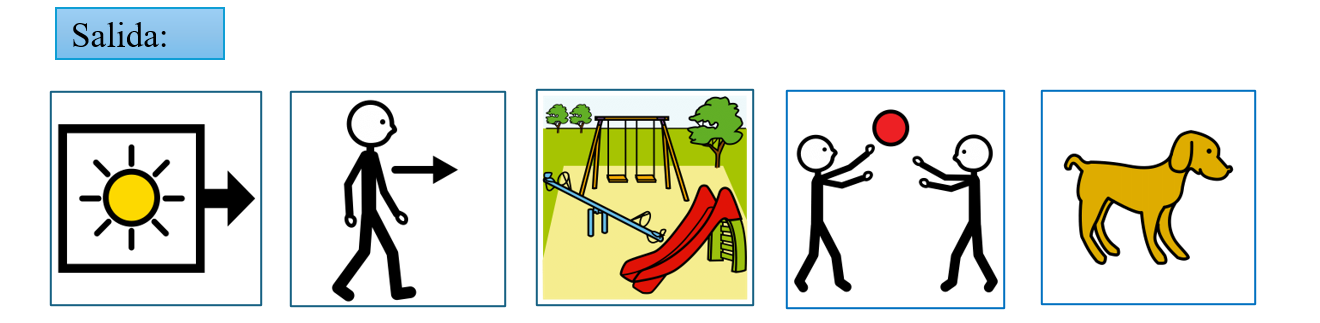
\includegraphics[width=0.75\textwidth]{img/ejemplo1.png}
    \caption{Ejemplo de secuencia de pictogramas}
    \label{fig:ejemplo de salida}
\end{figure}
El sistema no solo debe buscar las imágenes individuales que corresponden a cada palabra, sino sintetizar de forma óptima la estructura gramatical para presentar una secuencia coherente de pictogramas (véase la Figura~\ref{fig:ejemplo de salida}) que mantenga la intención semántica original del usuario.
\subsection{Justificación}
La comunicación constituye un derecho humano fundamental, sin embargo, su ejercicio pleno permanece inaccesible para las  personas que presentan discapacidades del lenguaje derivadas de condiciones como el autismo, la afasia, el síndrome de Rett o la parálisis cerebral. En México, el Instituto Nacional de Estadística y Geografía estima que más de más de 900 mil personas tienen una discapacidad para hablar o comunicarse \cite{inegi2020cpv}, por tal motivo es relevante desarrollar herramientas tecnológicas de apoyo accesibles y eficaces. La Comunicación Aumentativa y Alternativa (CAA), particularmente mediante el uso de pictogramas, representa una de las vías más consolidadas para atender esta necesidad \cite{beukelman2013}.

No obstante, los sistemas actuales de traducción automática de texto a pictogramas presentan limitaciones estructurales que restringen considerablemente su utilidad práctica. Herramientas como AraWord operan mediante mapeo léxico directo, ignorando el contexto de la oración \cite{araword2020}. Por su parte,  Text-to-Pictogram incorpora redes léxicas y técnicas de desambiguación de sentidos, pero pierde la coherencia global al procesar el texto de forma lineal y modular \cite{sevens2015}. Otra herramienta para este propósito, Aratraductor, si bien dio un paso importante al usar análisis sintáctico  para identificar lemas y  usar una técnica de N-grams para detectar frases hechas; este enfoque depende demasiado de reglas gramaticales fijas, lo cual impide su generalización y escalabilidad. Ninguno de estos enfoques es capaz de modelar de forma integral las dependencias semánticas de una oración, tampoco de manejar adecuadamente fenómenos como la polisemia, la negación o las expresiones idiomáticas. La raíz de estas deficiencias reside en su arquitectura: al ser sistemas modulares basados en reglas o recursos lingüísticos explícitos, carecen de la capacidad de aprender representaciones contextuales a partir de datos.

\subsection{Solución propuesta}
Frente a este panorama, el presente trabajo propone una arquitectura de aprendizaje profundo unificada, fundamentado en la arquitectura Transformer \cite{vaswani2017attention}. A diferencia de los modelos precedentes, esta aproximación aprovecha el mecanismo de \textit{self-attention} para modelar dependencias globales en la oración, permitiendo que la generación de cada pictograma considere el contexto semántico completo y no solo la unidad léxica inmediata. La adopción de modelos pre-entrenados como T5 o mT5 \cite{raffel2020}  permite transferir conocimiento lingüístico profundo hacia la tarea específica de traducción a pictogramas. La originalidad de la propuesta reside en dos ejes: la aplicación de arquitecturas Transformer para el modelado integral del contexto, y la validación mediante un diseño experimental que emplea métricas estandarizadas de traducción automática. Esto permitirá realizar una comparativa objetiva entre el enfoque propuesto y los sistemas tradicionales basados en reglas.

El sistema beneficiaría directamente a personas usuarias de CAA y a sus familias, cuidadores y terapeutas del lenguaje, así como a desarrolladores de aplicaciones de accesibilidad, e incluso a personas aprendiendo un segundo idioma. Su viabilidad es alta,  por la disponibilidad abierta de los pictogramas ARASAAC, así como también por el aporte del corpus en inglés de la tarea \textit{Text-to-Picto} de ImageCLEF 2026. ImageCLEF es un laboratorio de evaluación internacional que forma parte de la CLEF (Conference and Labs of the Evaluation Forum), una iniciativa europea centrada en la evaluación de sistemas de información, se lleva a cabo cada año desde 2003 \cite{unknown-author-no-date2}.

Desde una perspectiva académica, el proyecto abarca distintas áreas relevantes de la Ingeniería en Inteligencia Artificial. Lo anterior se logra al establecer un flujo de trabajo estructurado donde el procesamiento de lenguaje natural se usa para preparar los datos; luego apoyándose en el aprendizaje profundo, se entrena a un modelo Transformer, y finalmente las métricas de evaluación validan el éxito de los resultados. Al trabajar estas áreas como un conjunto unificado, el proyecto busca resultados técnicos confiables y un beneficio social real.

\subsection{Objetivo general}

Desarrollar un sistema de traducción automática de texto en lenguaje natural a secuencias de pictogramas ARASAAC, basado en arquitecturas de aprendizaje profundo (Transformers).





\subsection{Objetivos particulares}
\begin{enumerate}
    \item Construir un corpus  Español-Pictogramas a partir de los datos de la tarea \textit{Text-to-Picto} de ImageCLEF 2026, realizando la traducción  y la validación de la alineación semántica para el idioma español.
    \item Implementar un modelo \textit{encoder-decoder} basado en Transformers para la tarea de traducción texto a pictogramas.
    \item Evaluar el sistema propuesto utilizando métricas estándar de traducción automática.
    \item Desarrollar una interfaz de usuario web que consuma el modelo entrenado mediante una API, permitiendo la interacción en tiempo real y la visualización de las secuencias generadas.
\end{enumerate}


\subsection{Metodología}

La metodología del proyecto seguirá de manera adaptada y práctica las fases del modelo \textit{CRISP-ML}, orientadas a garantizar calidad, trazabilidad y reproducibilidad en el desarrollo de un sistema de traducción automática de texto a pictogramas. Cada fase indica las actividades, entregables y controles de calidad asociados.

\begin{enumerate}

    \item \textbf{Comprensión del problema y de los datos (\textit{Business \& Data Understanding})}

    En una primera etapa, se definirá con claridad el problema desde una perspectiva técnica y social. Se establecerán los objetivos funcionales del sistema, determinando que el modelo deberá traducir texto en español, y en otros cuatro idiomas (inglés, alemán, ruso y turco), a secuencias coherentes de identificadores de pictogramas de ARASAAC, preservando el significado semántico global del mensaje. En esta fase se evaluarán también los conjuntos de datos disponibles para la tarea y se seleccionará el que se ajuste al alcance del proyecto.

    Asimismo, se especificarán criterios de éxito medibles, tales como desempeño en métricas automáticas (\textit{SacreBLEU}, \textit{METEOR}, \textit{PictoER}), reducción de ambigüedades léxicas y tiempos de respuesta aceptables en la \textit{API} de inferencia. También se establecerán requisitos no funcionales relacionados con accesibilidad y reproducibilidad.

    \item \textbf{Ingeniería de datos (\textit{Data Engineering / Data Preparation})}

    Se partirá del corpus \textit{Propicto-Orfeo}, cuyos textos fuente en francés se traducirán a cinco idiomas con NLLB-200. Antes de traducir el corpus completo se verificará la calidad de la traducción mediante una prueba piloto evaluada con CometKiwi. Cada ejemplo se procesará de forma bidireccional (texto a identificadores e identificadores a texto). Posteriormente, se definirán dos configuraciones de vocabulario: una que conserva el tokenizador original del modelo y otra que agrega como tokens completos los identificadores de pictograma frecuentes.

    En paralelo, se definirá el vocabulario de salida correspondiente a los identificadores de pictogramas ARASAAC. Se estructurará el corpus en particiones de entrenamiento, validación y prueba, garantizando que todas las versiones de una misma oración (sus cinco traducciones y ambas direcciones) pertenezcan a la misma partición, para evitar filtraciones de información.

    \item \textbf{Ingeniería del modelo de aprendizaje automático (\textit{Machine Learning Model Engineering})}

    En la fase de modelado se ajustará un modelo de lenguaje \textit{decoder-only} preentrenado y multilingüe (Qwen3-4B) mediante LoRA, una técnica de ajuste eficiente que entrena solo un pequeño conjunto de parámetros adicionales. El modelo aprenderá a predecir directamente la secuencia de identificadores de pictogramas a partir del texto. Se compararán las dos configuraciones de vocabulario definidas en la fase anterior.

    Se establecerán configuraciones experimentales que incluirán selección de hiperparámetros, optimizador, tasa de aprendizaje y estrategias de regularización. Se utilizará validación temprana para prevenir sobreajuste y se almacenarán los pesos correspondientes a los mejores modelos obtenidos.

    Adicionalmente, se utilizará como línea base el traductor basado en reglas empleado en la construcción del corpus, con el fin de establecer una referencia cuantitativa que permita demostrar las mejoras aportadas por el enfoque neuronal.

    \item \textbf{Evaluación de los modelos (\textit{Evaluating Machine Learning Models})}

    El sistema entrenado será evaluado utilizando métricas estándar de traducción automática como \textit{SacreBLEU}, \textit{METEOR} y \textit{PictoER}. Las métricas se calcularán sobre las secuencias de identificadores de pictograma y, para comparar con los sistemas de ToPicto 2026, también sobre los términos obtenidos al convertir los identificadores mediante el léxico de ARASAAC.

    Los resultados se compararán con la línea base de reglas y con los sistemas reportados en ToPicto 2026, considerando que el modelo propuesto es de mayor tamaño, lo que limita la atribución de las mejoras únicamente al enfoque. A partir de esta comparación se establecerá una discusión crítica sobre ventajas y limitaciones del enfoque propuesto.

    \item \textbf{Despliegue (\textit{Deployment})}

    Una vez validado el modelo, se procederá a su integración en una arquitectura de servicio. El modelo será encapsulado en una \textit{API REST} que permitirá recibir texto en cualquiera de los cinco idiomas del corpus, generar directamente la secuencia de identificadores de ARASAAC y validar que existan en su catálogo.

    Posteriormente, se desarrollará una interfaz web que consumirá dicha \textit{API}, permitiendo al usuario introducir texto y visualizar de forma inmediata los pictogramas generados. La interfaz priorizará criterios de accesibilidad y claridad visual, asegurando facilidad de uso para usuarios finales. Las imágenes se obtendrán del servicio de ARASAAC y conservarán la atribución que exige su licencia CC BY-NC-SA.

    El sistema será empaquetado mediante tecnologías de contenedorización, lo que permitirá su despliegue reproducible en distintos entornos.

    \item \textbf{Monitoreo y mantenimiento (\textit{Monitoring and Maintenance})}

    Se monitoreará el modelo durante un periodo determinado para verificar su correcto funcionamiento mediante el análisis de métricas de desempeño, incluido el porcentaje de identificadores generados que no existen en el catálogo de ARASAAC. En caso de detectar anomalías o degradación en el rendimiento, se realizará el mantenimiento correspondiente.

\end{enumerate}

\subsection{Estructura del trabajo}
\section{Marco teórico conceptual}
\label{sec:marco-teorico}

En este capítulo se presentan los conceptos que sustentan el trabajo. Se parte del Procesamiento de Lenguaje Natural, su evolución y sus tareas principales, para ubicar a la traducción automática dentro del campo. Después se describe la Comunicación Aumentativa y Alternativa, el catálogo de pictogramas ARASAAC y la función comunicativa de la traducción de texto a pictogramas. Enseguida se explican las redes neuronales, la arquitectura Transformer y los modelos preentrenados, que son la base técnica del modelo propuesto. Finalmente, se aborda la traducción automática con Transformers y las métricas con las que se evalúa la calidad de una traducción, junto con su adaptación al caso de los pictogramas.

\subsection{Procesamiento de Lenguaje Natural (PLN)}
El Procesamiento de Lenguaje Natural (NLP, por sus siglas en inglés) es la disciplina de la Inteligencia Artificial dedicada a dotar a los sistemas computacionales de la capacidad de comprender, interpretar y generar lenguaje humano de forma automática \cite{bharadiya2023nlp}. 

    De acuerdo a Bharadiya\cite{bharadiya2023nlp}, los orígenes del procesamiento de lenguaje se remontan a enfoques basados en reglas lingüísticas explícitas, diseñadas manualmente por expertos, que buscaban capturar la gramática y la semántica del lenguaje mediante sistemas simbólicos. Con el tiempo, la disciplina evolucionó hacia paradigmas cada vez más dependientes de datos.

\subsubsection{Evolución metodológica del NLP}

La evolución del NLP ha ido cambiando de enfoque como respuesta a las limitaciones y nuevas necesidades. Por ejemplo,los primeros sistemas estaban basados en reglas y por ende dependían de gramáticas formales y diccionarios construidos manualmente por lingüistas computacionales; si bien permitían un control interpretable sobre el comportamiento del sistema, su escalabilidad era limitada, dado que la cobertura de fenómenos lingüísticos crecía linealmente con el esfuerzo humano requerido, y presentaban un mal desempeño frente a la ambigüedad y variabilidad inherentes al lenguaje natural.

Estas limitaciones impulsaron el desarrollo de métodos estadísticos que modelaban el lenguaje como distribuciones de probabilidad obtenidas a partir del análsisi de grandes volúmenes de texto, ejemplos de este paradigma son los modelos de m-gramas y los modelos ocultos de Markov. Sin embargo estos modelos seguían dependiendo en gran medida de ingeniería manual de características, como resultado se buscaron mejoras mediante la incorporación de técnicas de aprendizaje automático clásico y posteriormente de técnicas de aprendizaje profundo. Este último permite que los propios modelos aprendar representaciones a partir del texto de origen sin necesidad de ingeniería manual de características \cite{young2018recent}.

 Las arquitecturas neuronales demostraron una capacidad superior para capturar dependencias contextuales y relaciones semánticas complejas, lo que condujo, en años recientes, a la emergencia de modelos preentrenados sobre volúmenes masivos de texto y posteriormente adaptados a tareas específicas, así como al surgimiento de los denominados Large Language Models (LLM), capaces de exhibir capacidades emergentes de comprensión y generación de lenguaje a una escala sin precedentes en la historia del campo.


\subsubsection{Principales tareas del Procesamiento de Lenguaje Natural}

Hang Li \cite{Li2018} propone una clasificación de cinco tareas principales dentro del procesamiento de lenguaje natural, las cuales son clasificación (classification), emparejamiento (matching), traducción (translation), predicción estructurada (structured prediction) y proceso de decisión secuencial (sequential decision process). La  tabla \ref{tab:five-nlp-tasks} resume dichas tareas.

\begin{table}[H]
\centering
\caption{Cinco tareas del procesamiento de lenguaje natural \cite{Li2018}}
\label{tab:five-nlp-tasks}
\renewcommand{\arraystretch}{1.4}
\setlength{\tabcolsep}{8pt}
\small
\begin{tabular}{@{} >{\raggedright\arraybackslash}p{2.6cm}
                    >{\raggedright\arraybackslash}p{3.2cm}
                    >{\raggedright\arraybackslash}p{2.6cm}
                    >{\raggedright\arraybackslash}p{4.2cm} @{}}
\toprule
\textbf{Tarea} & \textbf{Descripción} & \textbf{Modelo} & \textbf{Aplicaciones} \\
\midrule

Clasificación &
asignar una etiqueta a una cadena &
$s \rightarrow c$ \newline
$s$: cadena, $c$: etiqueta &
clasificación de texto, análisis de sentimientos \\

\midrule

Emparejamiento &
comparar dos cadenas &
$s, t \rightarrow R^{+}$ \newline
$s$: cadena, $t$: cadena \newline
$R^{+}$: valores reales no negativos &
búsqueda, respuesta a preguntas, diálogo de un turno (basado en recuperación) \\

\midrule

Traducción &
transformar una cadena en otra &
$s \rightarrow t$ \newline
$s$: cadena, $t$: cadena &
traducción automática, reconocimiento automático de voz, diálogo de un turno (basado en generación) \\

\midrule

Predicción estructurada &
mapear una cadena a una estructura &
$s \rightarrow [s]$ \newline
$s$: cadena, $[s]$: estructura &
reconocimiento de entidades nombradas, segmentación de palabras, etiquetado gramatical, análisis de dependencias, análisis semántico \\

\midrule

Proceso de decisión secuencial &
tomar acciones en estados dentro de un entorno dinámicamente cambiante &
$\pi: s \rightarrow a$ \newline
$\pi$: política, $s$: estado, $a$: acción &
diálogo de múltiples turnos \\

\bottomrule
\end{tabular}
\end{table}


Entre estas tareas, la traducción automática ocupa un lugar particular por la complejidad que entraña: a diferencia de tareas de clasificación o etiquetado, que operan sobre un espacio de salida acotado, la traducción automática requiere generar una secuencia de salida completa en un espacio diferente. Además de que se debe de preservar simultáneamente el contenido semántico, la estructura sintáctica y las convenciones idiomáticas del idioma destino. 

\subsubsection{Representación computacional del lenguaje}

Para que el lenguaje natural pueda ser procesado por algoritmos, primero debe transformarse en representaciones numéricas. Una de las técnicas más simples es Bag of Words que usa vectores de frecuencia de palabras, ignorando orden y contexto, esta aproximación tiene la desventaja de que sufre alta dimensionalidad, dispersión y nula semántica \cite{murel2023bagofwords}. Otra técnica es TF-IDF, esta pondera por rareza en el corpus, mejorando la discriminación, pero sigue sin captar significado entre términos: por ejemplo, trata palabras como coche y automóvil como entidades completamente independientes, sin reconocer su relación semántica.

Word Embeddings introducen vectores densos y de baja dimensión que sitúan palabras relacionadas cerca, capturando relaciones semánticas y analógicas. Sin embargo, asignan una representación fija por palabra, sin adaptarse al contexto (problema de polisemia). Los embeddings contextuales generan representaciones dinámicas según la oración completa, resolviendo esto. Esta capacidad de capturar dependencias complejas y de largo alcance exige modelos que puedan procesar secuencias enteras y ponderar la influencia de cada elemento sobre los demás, lo cual se logra mediante arquitecturas neuronales profundas como las redes recurrentes, las convolucionales o, más recientemente, los \textit{transformers}; estas arquitecturas son precisamente las que permiten aprender los pesos y atenciones necesarios para producir embeddings sensibles al contexto, de modo que la necesidad de representar el significado variable de las palabras según su entorno es lo que ha impulsado la adopción generalizada de estos modelos en el NLP moderno.

\subsubsection{Aprendizaje profundo aplicado al NLP}
El Aprendizaje Profundo transformó el procesamiento de secuencias lingüísticas mediante arquitecturas capaces de modelar dependencias entre elementos distantes dentro de una secuencia. Las Redes Neuronales Recurrentes (RNN) fueron de las primeras arquitecturas adoptadas ampliamente para esta tarea, al procesar secuencias de forma iterativa mientras mantienen un estado oculto que resume la información previa; sin embargo, su capacidad para capturar dependencias de largo alcance se ve limitada por el problema del desvanecimiento del gradiente, este problema ocurre cuando los cambios que hacen que mejoren los parametros de una red, se vuelven demasiado pequeños \cite{ultralytics2026vanishing}. Las arquitecturas LSTM (Long Short-Term Memory) y GRU (Gated Recurrent Unit) surgieron como refinamientos de las RNN, incorporando mecanismos de compuertas que regulan el flujo de información y mitigan dicho problema, mejorando sustancialmente la capacidad de modelar contexto a mayor distancia dentro de una secuencia \cite{young2018recent}.

No obstante, estas arquitecturas recurrentes conservaban una limitación estructural: su naturaleza secuencial impedía la paralelización eficiente durante el entrenamiento y seguía dificultando el procesamiento de dependencias muy distantes. La incorporación de mecanismos de atención, que permiten a un modelo ponderar dinámicamente la relevancia de distintas posiciones de la secuencia de entrada al generar cada elemento de salida, fue uno de los intentos de mejora hacia la superación de esta limitación. Este principio fue posteriormente llevado a su expresión más influyente con la arquitectura Transformer, cuya importancia radica en haber prescindido por completo de la recurrencia, apoyándose únicamente en mecanismos de atención para modelar relaciones entre todos los elementos de una secuencia de forma paralela.

\subsubsection{Relación con la traducción automática}

La traducción automática constituye una de las aplicaciones más exigentes del Procesamiento de Lenguaje Natural, en la medida en que su resolución adecuada requiere la integración simultánea de múltiples niveles de análisis lingüístico. Un sistema de traducción competente debe capturar la sintaxis de ambos idiomas involucrados, resolver ambigüedades semánticas dependientes de contexto, mantener coherencia a lo largo de la secuencia generada, modelar las relaciones estructurales entre palabras y frases, y preservar el significado global del enunciado original al transformarlo en una representación equivalente dentro de un sistema lingüístico distinto. Esta naturaleza multidimensional convierte a la traducción automática en un caso de estudio particularmente representativo de los desafíos centrales del NLP, y motiva su desarrollo detallado más adelante en este capítulo, donde se abordan tanto su formulación como las arquitecturas neuronales que han definido su estado actual.


\vspace{0.5cm}
\subsection{Sistemas Pictográficos y Comunicación Aumentativa y Alternativa (CAA)}
\vspace{0.2cm}

Hay personas para quienes el habla o la escritura no bastan para comunicarse en la vida diaria. Beukelman y Light \cite{beukelman2020aac} se refieren a ellas como personas con \textit{necesidades complejas de comunicación}, un grupo amplio que incluye, entre otros, a niñas y niños con trastorno del espectro autista, parálisis cerebral o síndrome de Down, y a adultos que han perdido parte de su lenguaje después de un accidente cerebrovascular o por una enfermedad neurodegenerativa. Para este grupo se desarrolló la Comunicación Aumentativa y Alternativa (CAA), que reúne los sistemas, estrategias y herramientas que complementan el habla (aumentativa) o la sustituyen cuando no está disponible (alternativa) \cite{beukelman2020aac}.

Los recursos de CAA van desde gestos y tableros de papel hasta dispositivos electrónicos que reproducen voz sintetizada. Dentro de este abanico, los sistemas pictográficos ocupan un lugar central. Un pictograma es una imagen simplificada que representa un concepto (un objeto, una acción, una emoción o una persona) y que suele acompañarse de la palabra escrita correspondiente. Al combinar pictogramas en secuencia, la persona usuaria puede construir enunciados completos sin necesidad de leer o pronunciar cada palabra.

\begin{figure}[H]
    \centering
    \begin{subfigure}[b]{0.22\textwidth}
        \centering
        
\includegraphics[width=\textwidth]{img/pictos/2462-manzana.png}
        \caption{Objeto: \textit{manzana}}
        \label{fig:picto-objeto}
    \end{subfigure}
    \hfill
    \begin{subfigure}[b]{0.22\textwidth}
        \centering
        
\includegraphics[width=\textwidth]{img/pictos/6456-comer.png}
        \caption{Acción: \textit{comer}}
        \label{fig:picto-accion}
    \end{subfigure}
    \hfill
    \begin{subfigure}[b]{0.22\textwidth}
        \centering
        
\includegraphics[width=\textwidth]{img/pictos/35547-contento.png}
        \caption{Emoción: \textit{contento}}
        \label{fig:picto-emocion}
    \end{subfigure}
    \hfill
    \begin{subfigure}[b]{0.22\textwidth}
        \centering
        
\includegraphics[width=\textwidth]{img/pictos/2467-médico.png}
        \caption{Persona: \textit{médico}}
        \label{fig:picto-persona}
    \end{subfigure}
    \caption{Ejemplos de pictogramas de ARASAAC para distintos tipos de concepto \cite{arasaac}}
    \label{fig:pictos-individuales}
\end{figure}


\subsubsection{ARASAAC}

ARASAAC (Centro Aragonés para la Comunicación Aumentativa y Alternativa) es uno de los repositorios pictográficos más utilizados en el mundo hispanohablante. Fue creado por el Gobierno de Aragón y ofrece un catálogo de varios miles de pictogramas distribuidos bajo licencia Creative Commons (BY-NC-SA), con traducciones de sus términos a numerosos idiomas \cite{arasaac}. Cada pictograma tiene un identificador numérico único y uno o más términos asociados que representan diversos tipos de conceptos (véase la Figura~\ref{fig:pictos-individuales}), lo cual lo vuelve útil para el trabajo computacional: una secuencia de pictogramas puede tratarse como una secuencia de tokens tomados de un vocabulario cerrado. Precisamente por esa razón, ARASAAC es el catálogo de referencia de la tarea ImageCLEFtoPicto, en la que cada término pictográfico producido por un sistema debe corresponder a una imagen concreta del repositorio \cite{macaire2025overview}. Los pictogramas de ARASAAC que se muestran en este documento son obra de Sergio Palao, propiedad del Gobierno de Aragón, y se reproducen bajo la licencia CC BY-NC-SA \cite{arasaac}.


\subsubsection{Función comunicativa y relevancia de la traducción texto-pictograma}

Los pictogramas cumplen dos funciones que conviene separar. La primera es expresiva: permiten a la persona usuaria producir mensajes propios, por ejemplo al señalar en un tablero las imágenes de «yo», «querer» y «agua» (véase la Figura~\ref{fig:tablero}). La segunda es receptiva: ayudan a que la persona comprenda lo que otros le dicen, pues un enunciado acompañado de pictogramas resulta más accesible que el texto o el habla solos \cite{beukelman2020aac}.

\begin{figure}[h]
    \centering
    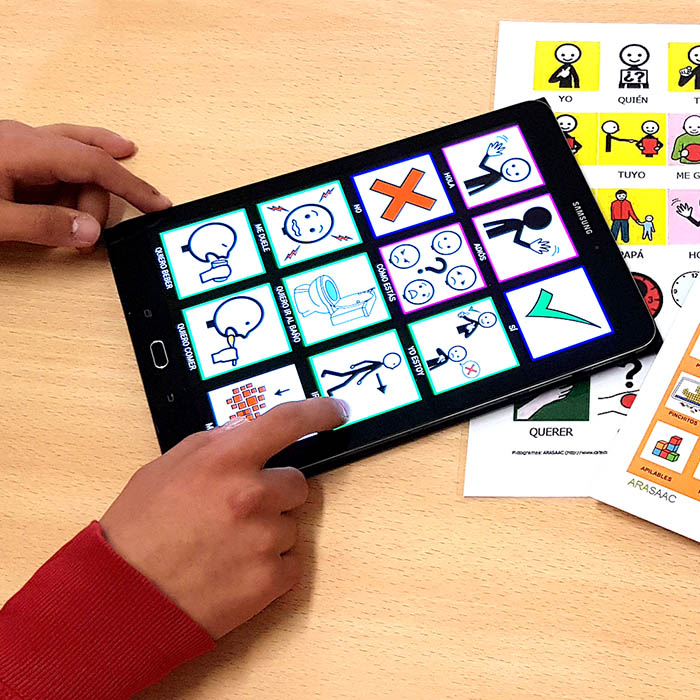
\includegraphics[width=0.45\textwidth]{img/pictos/tablero.jpg}
    \caption{Tablero de comunicación elaborado con pictogramas de ARASAAC. La persona usuaria señala los pictogramas en orden para formar un mensaje \cite{arasaac}}
    \label{fig:tablero}
\end{figure}

Esta segunda función es la que motiva la traducción automática de texto a pictogramas. En la práctica, preparar a mano una secuencia pictográfica para cada mensaje exige tiempo y conocimiento del catálogo, y eso limita la frecuencia con la que familiares, docentes o personal médico pueden usar pictogramas en una conversación real. Macaire et al.\ \cite{macaire2025overview} plantean la tarea Text-to-Picto justamente con este problema en mente: si un sistema es capaz de generar de forma automática una secuencia de pictogramas comprensible a partir de un enunciado, se facilita que la comunicación entre ambas partes se inicie sin depender de una preparación previa. En la edición 2025 de la tarea, además, se incorporaron enunciados del dominio médico junto con los de la vida cotidiana, lo cual refleja que uno de los escenarios de uso previstos es la comunicación entre pacientes y personal de salud.

\vspace{0.5cm}
\subsection{Redes Neuronales y Aprendizaje Profundo}
\vspace{0.2cm}

Una red neuronal artificial es un modelo compuesto por unidades de cálculo sencillas (neuronas) organizadas en capas. Cada neurona recibe un conjunto de entradas, calcula una suma ponderada de ellas, le agrega un sesgo y aplica una función de activación no lineal. Para una capa completa, esta operación se escribe de forma compacta como
\begin{equation}
\mathbf{h} = \sigma(\mathbf{W}\mathbf{x} + \mathbf{b}),
\end{equation}
donde $\mathbf{x}$ es el vector de entrada, $\mathbf{W}$ la matriz de pesos, $\mathbf{b}$ el vector de sesgos y $\sigma$ la función de activación (por ejemplo, ReLU o la tangente hiperbólica) \cite{goodfellow2016deep}. Sin la no linealidad, apilar capas equivaldría a aplicar una sola transformación lineal; es la función de activación la que permite que una red aproxime relaciones complejas entre entrada y salida.

Los pesos de la red no se diseñan a mano. Se ajustan a partir de ejemplos mediante la minimización de una función de pérdida que mide qué tan lejos está la predicción del valor esperado. El algoritmo que hizo práctico este ajuste en redes de varias capas fue la retropropagación del error, popularizada por Rumelhart, Hinton y Williams \cite{rumelhart1986learning}: el gradiente de la pérdida se calcula capa por capa, desde la salida hacia la entrada, aplicando la regla de la cadena, y luego se usa para actualizar los pesos con alguna variante del descenso por gradiente.


\subsubsection{Del aprendizaje superficial al profundo}


La idea de entrenar redes con muchas capas existía desde hace décadas, pero durante mucho tiempo resultó difícil llevarla a la práctica por falta de datos, de capacidad de cómputo y por problemas numéricos durante el entrenamiento. LeCun, Bengio y Hinton \cite{lecun2015deep} describen cómo esta situación cambió a partir de la década de 2010, cuando la disponibilidad de grandes conjuntos de datos, el uso de GPU y mejoras en inicialización y regularización permitieron entrenar redes profundas de forma estable. Lo que distingue al aprendizaje profundo, según estos autores, es que cada capa aprende una representación un poco más abstracta que la anterior, de modo que el modelo descubre por sí mismo las características relevantes que antes debían definirse manualmente.

En el caso del lenguaje, el reto particular es que los datos son secuencias de longitud variable en las que el orden importa. Las redes recurrentes atendieron este problema manteniendo un estado oculto que se actualiza con cada nuevo elemento, y las LSTM de Hochreiter y Schmidhuber \cite{hochreiter1997lstm} introdujeron compuertas que controlan qué información se conserva y cuál se descarta, lo que permitió aprender dependencias más largas que con una red recurrente simple. Como ya se describió en la sección anterior, estas arquitecturas dominaron el procesamiento de secuencias hasta la aparición de los mecanismos de atención y, después, del Transformer.


\subsubsection{Arquitectura Transformer}

El Transformer fue presentado por Vaswani et al.\ \cite{vaswani2017attention} en 2017 como un modelo de traducción automática que prescinde por completo de la recurrencia y de las convoluciones. En su lugar, cada posición de la secuencia se relaciona directamente con todas las demás mediante un mecanismo llamado autoatención (\textit{self-attention}). El trabajo mostró que esta arquitectura obtenía mejores resultados que los sistemas recurrentes de la época en las tareas de traducción inglés-alemán e inglés-francés de WMT 2014, con un costo de entrenamiento menor gracias a que las operaciones pueden paralelizarse.


\subsubsection{Atención de producto punto escalado}


La pieza básica del modelo es la atención de producto punto escalado. Cada token de la entrada se proyecta en tres vectores: una consulta ($q$), una clave ($k$) y un valor ($v$). Intuitivamente, la consulta expresa ``qué busca'' un token, la clave indica ``qué ofrece'' cada token y el valor es la información que efectivamente se transmite. Agrupando estos vectores en las matrices $Q$, $K$ y $V$, la atención se calcula como
\begin{equation}
\text{Attention}(Q, K, V) = \text{softmax}\left(\frac{QK^{\top}}{\sqrt{d_k}}\right)V,
\end{equation}
donde $d_k$ es la dimensión de las claves \cite{vaswani2017attention}. El producto $QK^{\top}$ mide la afinidad entre cada par de tokens, la función softmax convierte esas afinidades en pesos que suman uno, y el resultado es un promedio ponderado de los valores. La división entre $\sqrt{d_k}$ evita que los productos punto crezcan demasiado cuando la dimensión es grande, lo que llevaría a la softmax a regiones con gradientes muy pequeños.

En lugar de calcular una sola atención, el Transformer utiliza atención multicabeza: repite el cálculo anterior $h$ veces en paralelo con proyecciones distintas y concatena los resultados. Cada cabeza puede especializarse en un tipo de relación diferente, por ejemplo, una puede vincular un verbo con su sujeto y otra un pronombre con su referente.


\subsubsection{Codificador, decodificador y codificación posicional}


El modelo original sigue el esquema codificador-decodificador. El codificador está formado por una pila de capas idénticas, cada una con un bloque de autoatención multicabeza y una red \textit{feed-forward} aplicada a cada posición, ambos rodeados por conexiones residuales y normalización de capa. El decodificador tiene una estructura similar, con dos diferencias: su autoatención está enmascarada para que cada posición solo pueda ver los tokens ya generados, y añade un bloque de atención cruzada en el que las consultas provienen del decodificador y las claves y valores de la salida del codificador. Es en esta atención cruzada donde el modelo ``consulta'' la oración de origen mientras genera la de destino \cite{vaswani2017attention}.

Como la autoatención trata la entrada como un conjunto y no distingue el orden, los autores sumaron a cada embedding una codificación posicional construida con funciones seno y coseno de distintas frecuencias:
\begin{equation}
PE_{(pos, 2i)} = \sin\left(\frac{pos}{10000^{2i/d_{\text{model}}}}\right), \qquad
PE_{(pos, 2i+1)} = \cos\left(\frac{pos}{10000^{2i/d_{\text{model}}}}\right).
\end{equation}
De esta manera cada posición recibe una firma única y el modelo puede razonar sobre distancias relativas entre tokens \cite{vaswani2017attention}.

\vspace{0.5cm}
\subsection{Modelos Preentrenados y Transfer Learning}
\vspace{0.2cm}

El aprendizaje por transferencia (\textit{transfer learning}) parte de la noción de que, el conocimiento adquirido al resolver una tarea puede aprovecharse para resolver otra distinta pero relacionada. Pan y Yang \cite{pan2010survey} formalizan esta idea en términos de un dominio y una tarea de origen, de los que se extrae conocimiento, y un dominio y una tarea de destino, en los que se aplica. Su utilidad es mayor cuando la tarea de destino cuenta con pocos datos etiquetados, que es la situación habitual en problemas especializados.

En el procesamiento de lenguaje natural esta idea tomó la forma de un procedimiento en dos etapas. Primero, un modelo se \textit{preentrena} sobre grandes cantidades de texto sin etiquetar con un objetivo autosupervisado, como predecir palabras ocultas o la siguiente palabra. Después, ese mismo modelo se \textit{ajusta finamente} (\textit{fine-tuning}) con un conjunto de datos pequeño y etiquetado de la tarea que interesa. Uno de los trabajos que mostró que este esquema funcionaba en lenguaje natural fue ULMFiT (\textit{Universal Language Model Fine-tuning}), propuesto por Howard y Ruder \cite{howard2018ulmfit}. Su punto de partida es un modelo de lenguaje recurrente basado en LSTM, preentrenado sobre un corpus general extraído de Wikipedia para predecir la siguiente palabra. El método ajusta ese modelo en tres etapas: primero el preentrenamiento general, después un ajuste del modelo de lenguaje con texto del dominio de destino (aún sin etiquetas) y, por último, el ajuste como clasificador con los datos etiquetados. Con este procedimiento mostraron que con solo 100 ejemplos etiquetados se igualaba el desempeño de un modelo entrenado desde cero con cien veces más datos.


\subsubsection{Modelos preentrenados basados en Transformer}


La combinación del preentrenamiento con la arquitectura Transformer dio lugar a una familia de modelos que se convirtió en el punto de partida estándar del campo. BERT \cite{devlin2019bert} utiliza solo el codificador y se preentrena ocultando al azar una parte de los tokens de entrada para que el modelo los reconstruya a partir del contexto de ambos lados. Esto lo hace muy adecuado para tareas de comprensión, como clasificación o reconocimiento de entidades, pero no está pensado para generar texto.

Para tareas en las que la salida es una secuencia nueva, como la traducción, resultan más naturales los modelos que conservan el esquema completo codificador-decodificador. BART \cite{lewis2020bart} se preentrena corrompiendo el texto de entrada (borrando, enmascarando o desordenando fragmentos) y enseñando al modelo a recuperar el texto original. T5 \cite{raffel2020t5}, por su parte, parte de la propuesta de tratar cualquier problema de lenguaje como una conversión de texto a texto: la entrada es una cadena precedida por un prefijo que indica la tarea (por ejemplo, \textit{translate English to German:}) y la salida es otra cadena. Raffel et al.\ realizaron además un estudio sistemático comparando objetivos de preentrenamiento, arquitecturas y tamaños de modelo, lo que hizo de T5 una referencia útil para entender qué decisiones de diseño importan en la práctica. FLAN-T5 \cite{chung2022flan} extiende T5 con un ajuste adicional sobre una colección amplia de tareas formuladas como instrucciones, lo cual mejora su comportamiento cuando se enfrenta a tareas nuevas.

Estos modelos codificador-decodificador son relevantes para el presente trabajo porque son, en su mayoría, la base de los sistemas que han participado en la tarea Text-to-Picto, como se describe en el capítulo~\ref{sec:estado-arte}.

\vspace{0.5cm}
\subsection{Traducción Automática con Transformers}
\vspace{0.2cm}

La traducción automática neuronal formula el problema de traducir como el de modelar la probabilidad de una oración destino $\mathbf{y} = (y_1, \dots, y_m)$ dada una oración origen $\mathbf{x}$. Esta probabilidad se descompone de forma autorregresiva, es decir, cada token se predice a partir de la oración de origen y de los tokens ya generados:
\begin{equation}
P(\mathbf{y} \mid \mathbf{x}) = \prod_{t=1}^{m} P(y_t \mid y_{<t}, \mathbf{x}).
\end{equation}
Sutskever, Vinyals y Le \cite{sutskever2014sequence} mostraron que este esquema podía implementarse con dos redes LSTM, una que codifica la oración de origen en un vector de tamaño fijo y otra que genera la traducción a partir de él. El problema de comprimir toda la oración en un solo vector se hacía evidente con oraciones largas, y Bahdanau, Cho y Bengio \cite{bahdanau2015neural} lo atenuaron permitiendo que el decodificador consultara, en cada paso, una combinación ponderada de todos los estados del codificador. Ese mecanismo de atención es el antecedente directo del Transformer, que llevó la misma idea a todas las capas del modelo y eliminó la recurrencia \cite{vaswani2017attention}.


\subsubsection{Entrenamiento y decodificación}


Un modelo Transformer de traducción se entrena con pares de oraciones alineadas, minimizando la entropía cruzada entre la distribución que predice el modelo y el token correcto de la referencia en cada posición. Durante el entrenamiento se usa la técnica de \textit{teacher forcing}: el decodificador recibe como entrada los tokens verdaderos de la referencia y no los que él mismo generó, lo que permite procesar toda la oración en paralelo gracias a la máscara de atención.

Al momento de traducir ya no se dispone de la referencia, por lo que la salida debe construirse token por token. La estrategia más simple, la decodificación voraz, elige en cada paso el token más probable, pero puede comprometerse con una elección temprana que después resulte mala. Por ello es común usar búsqueda en haz (\textit{beam search}), que mantiene en paralelo las $k$ hipótesis parciales más probables y al final selecciona la de mayor probabilidad total \cite{sutskever2014sequence}.

Un último elemento práctico es el vocabulario. Los sistemas modernos no trabajan con palabras completas sino con unidades de subpalabra obtenidas con algoritmos como Byte Pair Encoding \cite{sennrich2016bpe} o SentencePiece. Esto permite representar palabras raras o nunca vistas como combinaciones de fragmentos conocidos, con un vocabulario de tamaño controlado.


\subsubsection{Relación con la traducción a pictogramas}

La traducción de texto a pictogramas puede plantearse con exactamente el mismo esquema: la oración de origen es el texto en lenguaje natural y la secuencia destino está formada por términos pictográficos de ARASAAC \cite{macaire2025overview}. Esto permite reutilizar modelos preentrenados como T5 o BART y ajustarlos con los pares texto-pictograma del conjunto de datos de la tarea.

Sin embargo, la adaptación tiene particularidades. El lenguaje de destino es más reducido que un idioma natural, ya que carece de flexiones y de la mayoría de las palabras funcionales, así que la tarea consiste en buena medida en decidir qué conceptos conservar, cómo normalizarlos a su forma canónica y en qué orden presentarlos. Además, el vocabulario de salida es cerrado, lo que abre la posibilidad de restringir la generación a términos que efectivamente existan en el catálogo.


\subsection{Métricas de Evaluación en Traducción Automática}
La evaluación de sistemas de Traducción Automática (MT, por sus siglas en inglés) constituye un componente metodológico indispensable para el avance del campo, dado que permite comparar de forma objetiva el desempeño de distintas arquitecturas y determinar el grado de proximidad entre una traducción generada por un sistema y una traducción de referencia producida por un humano. Históricamente, la evaluación humana ha sido considerada el estándar de referencia por su capacidad de capturar matices semánticos, fluidez y adecuación que resultan difíciles de cuantificar computacionalmente; sin embargo, este tipo de evaluación presenta limitaciones sustanciales: es costosa en tiempo y recursos, difícil de escalar a grandes volúmenes de datos, y susceptible a variabilidad, lo que termina por afectar su reproducibilidad \cite{lee2023survey}.

Estas limitaciones motivaron el desarrollo de métricas automáticas que aproximan el juicio humano mediante el análisis de similitud léxica, sintáctica o semántica entre la hipótesis generada por el sistema y una o más referencias. El auge de la arquitectura \textit{Transformer} y la consecuente mejora sustancial en la calidad de las traducciones producidas por sistemas neuronales han intensificado la necesidad de contar con métricas automáticas confiables que permitan monitorear el progreso del campo sin depender exclusivamente de evaluación humana \cite{lee2023survey}. No obstante, evaluar y comparar sistemas de MT de forma automática continúa siendo una tarea no trivial: diversas métricas tradicionales, entre ellas BLEU y TER, han mostrado un desempeño limitado para capturar similitud semántica entre las salidas de los sistemas y las referencias humanas, lo cual ha impulsado tanto el refinamiento de métricas léxicas como el desarrollo de métricas basadas en representaciones neuronales \cite{lee2023survey}. Pese a estas limitaciones, las métricas automáticas basadas en superposición léxica mantienen vigencia dentro de la investigación en MT por su bajo costo computacional, su interpretabilidad y la posibilidad de comparabilidad directa con resultados reportados en trabajos previos.


\subsubsection{Relación con la traducción automática a pictogramas}


La traducción automática a pictogramas comparte con la MT convencional su formulación fundamental como un problema de \textit{sequence-to-sequence}: esto quiere decir que dado un enunciado de entrada, el sistema debe producir una secuencia de salida que preserve el contenido semántico del origen. En consecuencia, los desafíos de evaluación inherentes a la MT se trasladan directamente a la evaluación de sistemas de traducción a pictogramas.

Existen, sin embargo, diferencias sustanciales entre ambas tareas que condicionan la aplicabilidad directa de las métricas de MT. En primer lugar, el espacio de salida en la traducción a pictogramas no es lenguaje natural sino una secuencia de tokens discretos, cada uno vinculado a un pictograma perteneciente a un vocabulario cerrado (por ejemplo, el catálogo ARASAAC), lo cual reduce la variabilidad morfológica y sintáctica presente en el texto libre. En segundo lugar, los pictogramas no cambian de forma según el género, número o tiempo verbal (por ejemplo, no existe una versión distinta de un pictograma para «corrió» frente a «correrá»), y tampoco incluyen palabras funcionales como artículos, preposiciones o conjunciones («el», «de», «y»). Esto significa que aspectos que en la traducción automática de texto son muy importantes de evaluar (tales como el orden de las palabras o que las palabras concuerden entre sí en género y número) tienen una relevancia distinta cuando se trata de evaluar secuencias de pictogramas.

Pese a estas diferencias, resulta razonable adaptar las métricas originalmente diseñadas para MT a la tarea de traducción a pictogramas, dado que ambas comparten la necesidad de cuantificar la distancia entre una secuencia generada y una secuencia de referencia mediante superposición de unidades (n-gramas, tokens o ediciones). La principal ventaja de esta adaptación es la posibilidad de aprovechar métricas ya validadas y ampliamente adoptadas por la comunidad de MT, lo que favorece la comparabilidad de resultados entre sistemas. La principal limitación radica en que estas métricas fueron diseñadas y calibradas sobre corpus de lenguaje natural, por lo que su correlación con juicios humanos de calidad en el dominio pictográfico no está garantizada de forma automática y debe complementarse, como se discutirá más adelante, con métricas diseñadas específicamente para operar sobre el vocabulario pictográfico.

\subsubsection{BLEU}
\vspace{-0.1cm}
\begin{itemize}
\item \textit{Fundamentos} \\
\vspace{-0.5cm}

BLEU (Bilingual Evaluation Understudy) fue propuesta por \citet{papineni2002bleu} como respuesta a la necesidad de una métrica automática, rápida y de bajo costo que correlacionara razonablemente con el juicio humano, evitando la dependencia de evaluación manual extensiva. La motivación central de BLEU es que una traducción automática será considerada de mayor calidad en la medida en que comparta más n-gramas contiguos con una o varias traducciones de referencia producidas por humanos.

\item \textit{Funcionamiento}\\
\vspace{-0.5cm}

El cálculo de BLEU parte de la tokenización de la hipótesis y de la(s) referencia(s). Sobre el texto tokenizado se extraen n-gramas de orden $1$ a $N$ (típicamente $N=4$). Para cada orden $n$, se calcula la \textit{precisión de n-gramas modificada} ($p_n$), la cual difiere de la precisión estándar en que el conteo de coincidencias de cada n-grama se \textit{recorta} (clipping) al número máximo de veces que dicho n-grama aparece en cualquiera de las referencias, evitando así que un sistema obtenga una puntuación artificialmente alta repitiendo n-gramas de alta frecuencia.

Dado que la precisión de n-gramas tiende a favorecer traducciones más cortas que la referencia (al reducir la probabilidad de introducir n-gramas no coincidentes), BLEU incorpora una \textit{penalización por brevedad} (Brevity Penalty, BP) que castiga hipótesis sustancialmente más cortas que la referencia.

\item\textit{Formulación matemática} \\
\vspace{-0.5cm}

La precisión de n-gramas modificada se define como:

\begin{equation}
p_n = \frac{\sum_{C \in \{\text{Candidatos}\}} \sum_{n\text{-grama} \in C} \text{Count}_{\text{clip}}(n\text{-grama})}{\sum_{C' \in \{\text{Candidatos}\}} \sum_{n\text{-grama}' \in C'} \text{Count}(n\text{-grama}')}
\end{equation}

donde $\text{Count}_{\text{clip}}$ es el conteo de coincidencias recortado al máximo número de ocurrencias del n-grama en cualquier referencia. La penalización por brevedad se define como:

\begin{equation}
BP =
\begin{cases}
1 & \text{si } c > r \\
e^{(1 - r/c)} & \text{si } c \leq r
\end{cases}
\end{equation}

donde $c$ es la longitud de la hipótesis y $r$ es la longitud efectiva de la referencia (usualmente la de longitud más cercana a $c$). Finalmente, BLEU se calcula como:

\begin{equation}
\text{BLEU} = BP \cdot \exp\left(\sum_{n=1}^{N} w_n \log p_n\right)
\end{equation}

con $w_n$ los pesos asignados a cada orden de n-grama, típicamente uniformes ($w_n = 1/N$) \cite{papineni2002bleu}.

\item \textit{Ejemplo detallado} \\
\vspace{-0.5cm}

Sea la referencia: \textit{``el gato está sobre la alfombra''} y la hipótesis: \textit{``el gato está en la alfombra''}.

Para unigramas ($n=1$): la hipótesis tiene 6 tokens; de estos, coinciden con la referencia (con clipping) 5 (\textit{el, gato, está, la, alfombra}), por lo que $p_1 = 5/6$.

Para bigramas ($n=2$): los bigramas de la hipótesis son (el-gato, gato-está, está-en, en-la, la-alfombra); de estos coinciden con la referencia (el-gato, gato-está, la-alfombra), es decir 3 de 5, por lo que $p_2 = 3/5$.

Continuando de forma análoga para $n=3$ y $n=4$, y dado que $c = r = 6$ (BP = 1 pues $c = r$, no $c < r$), el valor final de BLEU se obtiene promediando geométricamente los $p_n$ ponderados y multiplicando por BP. Este ejemplo ilustra cómo un solo token distinto (``en'' en lugar de ``sobre'') degrada progresivamente más la puntuación conforme aumenta el orden del n-grama, ya que afecta a más n-gramas contiguos.

\item \textit{Interpretación} \\
\vspace{-0.5cm}

BLEU se expresa típicamente en una escala de 0 a 100 (o 0 a 1). Valores cercanos a 100 indican alta coincidencia léxica con la referencia; en la práctica, puntuaciones por encima de 30 suelen considerarse indicativas de una traducción comprensible, mientras que puntuaciones por encima de 50 se asocian con traducciones de alta calidad, aunque estos umbrales varían considerablemente según el par de idiomas y el dominio.

\item \textit{Ventajas}\\
\vspace{-0.5cm}

BLEU es computacionalmente eficiente, no requiere entrenamiento ni recursos lingüísticos adicionales, y ha sido validada extensamente por su correlación razonable con juicios humanos a nivel de corpus, lo que ha consolidado su uso como métrica de referencia en la literatura de MT durante más de dos décadas.

\item \textit{Limitaciones} \\
\vspace{-0.5cm}

BLEU no captura equivalencia semántica (penaliza sinónimos y paráfrasis válidas), es sensible a la tokenización empleada (lo cual compromete la reproducibilidad entre estudios si no se estandariza) \cite{lee2023survey}, y su correlación con juicios humanos es más débil a nivel de oración individual que a nivel de corpus completo.

\item \textit{Aplicación a traducción de pictogramas}\\
\vspace{-0.5cm}

En el contexto de traducción a pictogramas, BLEU puede aplicarse directamente sobre la secuencia de tokens pictográficos (en lugar de palabras), tratando cada identificador de pictograma como una unidad léxica. Esto permite capturar coincidencias exactas de secuencias de pictogramas, pero hereda la limitación de no reconocer equivalencias semánticas entre pictogramas distintos que podrían transmitir un significado similar dentro del vocabulario ARASAAC.
\end{itemize}


\subsubsection{METEOR}

\begin{itemize}
\item \textit{Fundamentos} \\
\vspace{-0.5cm}

METEOR (Metric for Evaluation of Translation with Explicit ORdering) fue propuesta por \citet{banerjee2005meteor} para abordar limitaciones específicas de BLEU, particularmente su insensibilidad al orden de palabras a nivel de oración y su incapacidad de reconocer coincidencias no exactas (sinónimos, variantes morfológicas). La motivación central es construir una métrica que se correlacione mejor con el juicio humano combinando precisión y \textit{recall}, en lugar de basarse exclusivamente en precisión de n-gramas.

\item \textit{Funcionamiento} \\
\vspace{-0.5cm}

METEOR alinea unigramas entre hipótesis y referencia mediante un proceso de emparejamiento en etapas sucesivas: primero coincidencias exactas, después coincidencias tras normalización morfológica (\textit{stemming}), y finalmente coincidencias de sinónimos mediante recursos léxicos externos (como WordNet, en la versión original para inglés). A partir del conjunto de unigramas alineados se calculan precisión ($P$) y \textit{recall} ($R$), que se combinan en una media armónica ponderada. Adicionalmente, METEOR agrupa los unigramas alineados en \textit{chunks} (bloques contiguos y ordenados de igual manera en ambas secuencias) y penaliza la fragmentación excesiva, capturando así, de forma indirecta, el orden de palabras.

\item \textit{Formulación matemática}\\
\vspace{-0.5cm}

La media armónica ponderada (F-mean), con fuerte sesgo hacia el recall, se define como:

\begin{equation}
F_{\text{mean}} = \frac{10 \cdot P \cdot R}{R + 9P}
\end{equation}

correspondiente al caso en que el parámetro $\alpha = 0.9$ en la forma general $F_{\text{mean}} = \frac{P \cdot R}{\alpha P + (1-\alpha) R}$. La penalización por fragmentación se calcula como:

\begin{equation}
\text{Penalty} = \gamma \left(\frac{ch}{m}\right)^{\beta}
\end{equation}

donde $ch$ es el número de \textit{chunks}, $m$ es el número total de unigramas alineados, y $\gamma$, $\beta$ son parámetros ajustables (comúnmente $\gamma = 0.5$, $\beta = 3$) \cite{banerjee2005meteor}. El puntaje final es:

\begin{equation}
\text{METEOR} = F_{\text{mean}} \cdot (1 - \text{Penalty})
\end{equation}


\item \textit{Ejemplo detallado} \\
\vspace{-0.5cm}

Retomando el ejemplo anterior: referencia \textit{``el gato está sobre la alfombra''} (6 unigramas) e hipótesis \textit{``el gato está en la alfombra''} (6 unigramas). Los unigramas alineados exactamente son 5 (\textit{el, gato, está, la, alfombra}), por lo que $P = 5/6$ y $R = 5/6$. Aplicando la fórmula de $F_{\text{mean}}$ con estos valores iguales, $F_{\text{mean}} = 5/6 \approx 0.833$. Dado que los unigramas alineados forman en su mayoría un único chunk contiguo (con una pequeña discontinuidad en el punto donde ``en'' reemplaza a ``sobre''), la penalización por fragmentación resulta baja, de modo que el puntaje final se aproxima a $F_{\text{mean}}$, quedando ligeramente por debajo de 0.833 tras aplicar la penalización.

\item \textit{Interpretación} \\
\vspace{-0.5cm}

METEOR se reporta en una escala de 0 a 100 (o 0 a 1); valores más altos indican mayor calidad de traducción. A diferencia de BLEU, sus valores tienden a ser numéricamente más altos para una misma traducción debido al sesgo hacia recall y al reconocimiento de coincidencias no exactas, por lo que los umbrales de referencia no son directamente comparables entre ambas métricas.

\item \textit{Ventajas} \\
\vspace{-0.5cm}


METEOR incorpora información semántica adicional no capturada por BLEU y considera explícitamente el orden de palabras mediante la penalización por fragmentación, lo cual mejora su correlación con juicios humanos a nivel de oración \cite{lee2023survey}.

\item \textit{Limitaciones} \\
\vspace{-0.5cm}

La dependencia de recursos léxicos externos (como WordNet) limita su aplicabilidad directa a idiomas o dominios donde dichos recursos son escasos o inexistentes; además, los parámetros $\alpha$, $\gamma$ y $\beta$ requieren calibración específica por idioma para un desempeño óptimo.

\item \textit{Aplicación a traducción de pictogramas} \\
\vspace{-0.5cm}

Aplicar METEOR a secuencias de pictogramas requiere redefinir la noción de ``sinónimo'' en términos del vocabulario pictográfico, dado que no existe un recurso léxico equivalente a WordNet para pictogramas ARASAAC. En ausencia de dicho recurso, la aplicación práctica de METEOR en este dominio suele limitarse a coincidencias exactas de identificadores de pictograma, lo que reduce su ventaja teórica frente a BLEU pero conserva su capacidad de penalizar fragmentación en el orden de la secuencia.
\end{itemize}

\subsubsection{TER}
\vspace{-0.1cm}
\begin{itemize}
\item \textit{Fundamentos} \\
\vspace{-0.5cm}

TER (Translation Edit Rate) fue propuesta por \citet{snover2006ter} con la motivación de cuantificar directamente el esfuerzo humano requerido para corregir una traducción automática hasta que coincida con una referencia, en lugar de medir superposición de n-gramas. Esta orientación hace de TER una métrica particularmente interpretable en contextos de posedición.

\item \textit{Funcionamiento} \\
\vspace{-0.5cm}

TER calcula el número mínimo de operaciones de edición (inserciones, eliminaciones, sustituciones y desplazamientos de bloques de palabras) necesarias para transformar la hipótesis en la referencia, mediante una variante del algoritmo de distancia de edición de Levenshtein extendida con la operación de desplazamiento (\textit{shift}), que permite reordenar secuencias completas de palabras con un costo unitario, reconociendo que distintos órdenes de palabras pueden ser igualmente válidos en muchos idiomas \cite{snover2006ter}.

\item \textit{Formulación matemática} \\
\vspace{-0.5cm}

\begin{equation}
\text{TER} = \frac{\text{\footnotesize No. de ediciones (inserciones + eliminaciones + sustituciones + desplazamientos)}}{\text{\footnotesize Número promedio de palabras en la(s) referencia(s)}}
\end{equation}

 A diferencia de BLEU y METEOR, TER es una métrica de \textit{error}, por lo que valores más bajos indican mejor calidad de traducción.

\item \textit{Ejemplo detallado} \\
\vspace{-0.5cm}

Con el mismo par (referencia de 6 palabras, hipótesis con una sustitución: ``en'' por ``sobre''), se requiere una única operación de edición (sustitución) para transformar la hipótesis en la referencia. Por lo tanto:

\begin{equation}
\text{TER} = \frac{1}{6} \approx 0.167 \; (16.7\%)
\end{equation}

lo que indica que, en promedio, un 16.7\% de las palabras de la referencia requirieron edición para reconstruirse a partir de la hipótesis.

\item \textit{Interpretación} \\
\vspace{-0.5cm}

Al ser una métrica de error, valores cercanos a 0 indican traducciones que requieren mínima edición (alta calidad), mientras que valores cercanos o superiores a 1 indican que la hipótesis requiere un número de ediciones comparable o mayor a la longitud total de la referencia.

\item \textit{Ventajas} \\
\vspace{-0.5cm}

TER es intuitivamente interpretable en términos de esfuerzo de posedición y su variante orientada a humanos (HTER) ha mostrado una correlación con juicios humanos comparable o superior a la de un segundo juicio humano independiente \cite{snover2006ter}.

\item \textit{Limitaciones} \\
\vspace{-0.5cm}

TER, al igual que BLEU, opera a nivel de superposición léxica exacta y no reconoce sinónimos o paráfrasis; además, el costo computacional del cálculo de la operación de desplazamiento es superior al de una distancia de edición estándar.


\item \textit{Aplicación a traducción de pictogramas}


TER resulta directamente aplicable a secuencias de pictogramas al tratar cada identificador de pictograma como una unidad editable, y su naturaleza basada en operaciones de edición la aproxima conceptualmente a PictoER, una métrica derivada de Word Error Rate y adoptada específicamente en la evaluación de sistemas de traducción a pictogramas, que desplaza la unidad de análisis de la palabra al token pictográfico para capturar con mayor precisión el tipo de error relevante en este dominio.
\end{itemize}


\subsubsection{chrF y chrF++}
\label{par:chrf}
\vspace{-0.1cm}
\begin{itemize}
\item \textit{Fundamentos} \\
\vspace{-0.5cm}
 
chrF (\textit{character n-gram F-score}) fue propuesta por \citet{popovic2015chrf} como una métrica automática que compara la hipótesis y la referencia a nivel de caracteres, no de palabras. La motivación es que BLEU trata como error total a dos palabras que solo difieren en una terminación, como \textit{gato} y \textit{gatos}. Al trabajar con caracteres, chrF reconoce coincidencias parciales, lo que la hace más adecuada para idiomas con mucha variación morfológica. Más tarde, \citet{popovic2017chrfpp} propuso chrF++, que añade a los n-gramas de caracteres los unigramas y bigramas de palabras.
 
\item \textit{Funcionamiento} \\
\vspace{-0.5cm}
 
Se extraen los n-gramas de caracteres de la hipótesis y de la referencia, normalmente de orden 1 a 6, sin contar los espacios. Para cada orden se calcula la precisión (qué parte de los n-gramas de la hipótesis aparece en la referencia) y el \textit{recall} (qué parte de los n-gramas de la referencia aparece en la hipótesis). Después se promedian los valores de todos los órdenes y se combinan en una F-score que da más peso al \textit{recall}. En chrF++ se hace lo mismo, pero también se incluyen n-gramas de palabras de orden 1 y 2.
 
\item \textit{Formulación matemática} \\
\vspace{-0.5cm}
 
Sean $\text{chrP}$ y $\text{chrR}$ la precisión y el \textit{recall} promedio de los n-gramas considerados. La métrica es:
 
\begin{equation}
\text{chrF}_{\beta} = (1+\beta^2)\,\frac{\text{chrP} \cdot \text{chrR}}{\beta^2 \cdot \text{chrP} + \text{chrR}}
\end{equation}
 
donde $\beta$ indica cuántas veces más importa el \textit{recall} que la precisión. El valor usual es $\beta = 2$ \cite{popovic2015chrf}. chrF++ usa la misma fórmula, pero el promedio incluye los n-gramas de caracteres de orden 1 a 6 y los de palabras de orden 1 a 2 \cite{popovic2017chrfpp}.
 
\item \textit{Ejemplo detallado} \\
\vspace{-0.5cm}
 
Sea la referencia \textit{``gato''} y la hipótesis \textit{``gatos''}. Para simplificar, se usan solo bigramas de caracteres. La referencia tiene 3 bigramas (\textit{ga, at, to}) y la hipótesis tiene 4 (\textit{ga, at, to, os}). Coinciden 3, por lo que la precisión es $3/4 = 0.75$ y el \textit{recall} es $3/3 = 1$. Con $\beta = 2$:
 
\begin{equation}
\text{chrF}_2 = 5 \cdot \frac{0.75 \cdot 1}{4 \cdot 0.75 + 1} = \frac{3.75}{4} \approx 0.94
\end{equation}
 
A nivel de palabra, BLEU no encontraría ninguna coincidencia entre \textit{gato} y \textit{gatos}. chrF, en cambio, reconoce que la hipótesis es casi correcta.
 
\item \textit{Interpretación} \\
\vspace{-0.5cm}
 
chrF++ se reporta en una escala de 0 a 100. Valores más altos indican que la hipótesis se parece más a la referencia. Como BLEU, sus valores solo son comparables entre sistemas evaluados sobre el mismo idioma y el mismo conjunto de prueba.
 
\item \textit{Ventajas} \\
\vspace{-0.5cm}
 
No depende de la tokenización en palabras, reconoce variantes morfológicas y no necesita recursos lingüísticos externos. Por eso se usa para reportar resultados en conjuntos con muchos idiomas, como FLORES-200 \cite{nllbteamNoLanguageLeft2022}.
 
\item \textit{Limitaciones} \\
\vspace{-0.5cm}
 
Sigue midiendo parecido superficial: no reconoce sinónimos ni paráfrasis. Además, sus valores dependen del sistema de escritura. En idiomas que no separan las palabras con espacios, como el japonés o el chino, los valores son mucho más bajos aunque la traducción sea buena, por lo que no sirve para comparar la calidad entre idiomas con escrituras distintas.
 
    
\end{itemize}
 
 
\subsubsection{CometKiwi}
\label{par:cometkiwi}
\vspace{-0.1cm}
\begin{itemize}
\item \textit{Fundamentos} \\
\vspace{-0.5cm}
 
CometKiwi fue propuesta por \citet{rei2022cometkiwi} como una métrica de \textit{estimación de calidad} (\textit{quality estimation}). A diferencia de BLEU, METEOR, TER o chrF++, no necesita una traducción de referencia: estima qué tan buena es una traducción usando solo la oración fuente y la traducción. La motivación es que en muchos casos reales no existen traducciones humanas con las cuales comparar, y aun así se necesita saber si una traducción automática es confiable.
 
\item \textit{Funcionamiento} \\
\vspace{-0.5cm}
 
CometKiwi es una red neuronal basada en un codificador Transformer multilingüe preentrenado. La oración fuente y su traducción se unen en una sola entrada y el codificador las procesa juntas, de modo que puede relacionar cada parte de la traducción con la parte correspondiente del original. La representación resultante pasa por una red \textit{feed-forward} que produce un solo número: la calidad estimada. El modelo se entrenó para imitar calificaciones que asignaron evaluadores humanos a miles de traducciones (\textit{direct assessments}) \cite{rei2022cometkiwi}.
 
\item \textit{Formulación matemática} \\
\vspace{-0.5cm}
 
Sea $s$ la oración fuente y $t$ su traducción. El codificador produce una representación conjunta $\mathbf{h} = \text{Enc}([s; t])$, y la calidad estimada es:
 
\begin{equation}
\hat{y} = \text{FFN}(\mathbf{h})
\end{equation}
 
Durante el entrenamiento se minimiza el error cuadrático medio entre $\hat{y}$ y la calificación humana $y$:
 
\begin{equation}
\mathcal{L} = \frac{1}{M}\sum_{i=1}^{M}\left(\hat{y}_i - y_i\right)^2
\end{equation}
 
donde $M$ es el número de pares de entrenamiento.
 
\item \textit{Ejemplo detallado} \\
\vspace{-0.5cm}
 
Sea la fuente en francés \textit{``le chat est sur le tapis''}. Si la traducción al español es \textit{``el gato está sobre la alfombra''}, el modelo reconoce que el contenido se conserva y asigna un valor alto. Si la traducción es \textit{``el gato está''}, el modelo detecta que falta información del original y asigna un valor más bajo, aunque lo que sí se tradujo sea correcto. Esto no se puede medir con chrF++ sin una traducción de referencia.
 
\item \textit{Interpretación} \\
\vspace{-0.5cm}
 
La versión \texttt{wmt22-cometkiwi-da} produce valores aproximadamente entre 0 y 1; valores más altos indican mayor calidad estimada. Como el modelo evalúa el significado y no la forma escrita, sus valores sí se pueden comparar entre idiomas con sistemas de escritura distintos.
 
\item \textit{Ventajas} \\
\vspace{-0.5cm}
 
No necesita referencias, captura equivalencias de significado (sinónimos, paráfrasis, cambios de orden) y funciona para los idiomas que cubre su codificador multilingüe.
 
\item \textit{Limitaciones} \\
\vspace{-0.5cm}
 
Su resultado no es interpretable: da un número, pero no explica qué error encontró. Requiere una GPU para evaluar volúmenes grandes de texto. Además, es menos confiable con oraciones muy cortas, porque tiene poco contexto para juzgar.

\end{itemize}

\section{Estado del arte}
\label{sec:estado-arte}

En este capítulo se revisan los trabajos previos sobre traducción automática de texto a pictogramas. La revisión se organiza en dos partes. La primera recorre la evolución de la tarea: desde los primeros sistemas basados en reglas y recursos léxicos, pasando por su formulación como traducción automática neuronal, hasta la creación de un corpus y una tarea compartida que hoy sirven como referencia común. La segunda parte analiza los sistemas más recientes, presentados en la tarea ImageCLEFtoPicto, y compara su desempeño con las mismas métricas con las que se evaluará el presente trabajo. Al final de cada parte, los hallazgos se sintetizan en una tabla.

\subsection{Evolución de la traducción de texto a pictogramas}

El primer planteamiento del problema como una tarea de traducción se encuentra en el trabajo de Mihalcea y Leong \cite{mihalcea2008}. Su sistema traducía oraciones simples en inglés a secuencias de imágenes obtenidas de motores de búsqueda y de colecciones de \textit{clipart}\footnote{\textit{Clipart}: colecciones de ilustraciones prediseñadas, generalmente dibujos sencillos, que se distribuyen listas para insertarse en documentos.}. Para evaluarlo, midieron qué tanto comprendían los lectores el mensaje a partir de las imágenes y lo compararon con la comprensión lograda con la salida de un sistema de traducción automática; la representación visual alcanzó un nivel de comprensión comparable. Este trabajo mostró que una secuencia de imágenes puede transmitir el contenido de una oración, aunque las imágenes no provenían de un sistema de CAA, el sistema se limitaba a oraciones simples y la evaluación no incluyó a personas con dificultades del lenguaje.

La primera línea de trabajo dirigida específicamente a la CAA es Text2Picto, de Vandeghinste et al.\ \cite{vandeghinste2017}. Este sistema convierte texto en neerlandés a los conjuntos pictográficos Sclera y Beta\footnote{Sclera y Beta son dos colecciones de pictogramas usadas en CAA en Bélgica y los Países Bajos. Sclera está formada por pictogramas sencillos en blanco y negro, mientras que Beta emplea dibujos a color.} mediante reglas: realiza un análisis lingüístico superficial del texto, consulta los \textit{synsets}\footnote{Un \textit{synset} (del inglés \textit{synonym set}) es un grupo de palabras que comparten un mismo significado; por ejemplo, «coche» y «automóvil». Es la unidad básica de WordNet y de bases léxicas similares, en las que cada \textit{synset} se enlaza con otros mediante relaciones de significado.} de las palabras de contenido en la base léxica Cornetto\footnote{Cornetto es una base de datos léxica del neerlandés, organizada en \textit{synsets} de forma similar a WordNet.} y busca el pictograma semánticamente más cercano. Al apoyarse en relaciones semánticas, puede representar palabras que no tienen un pictograma propio, y su comportamiento es interpretable sin necesidad de un corpus paralelo. Se evaluó frente a una línea base que buscaba coincidencias entre el texto y los nombres de archivo de los pictogramas. Su principal costo es que cada pictograma debe enlazarse manualmente con la base léxica, la traducción se realiza palabra por palabra y la desambiguación de sentidos es limitada.

Sevens et al.\ \cite{sevens2015} extendieron Text2Picto al inglés y al español reutilizando la misma arquitectura basada en recursos léxico-semánticos. Al comparar su desempeño con el del sistema original en neerlandés, mostraron que el enfoque se transfiere entre idiomas, y este fue el primer Text2Picto con entrada en inglés y en español, aunque todavía con los conjuntos Sclera y Beta y con las limitaciones propias de las reglas.

En el ámbito hispanohablante, Aratraductor \cite{bautista2017} traduce texto en español a pictogramas de ARASAAC e incorpora técnicas de procesamiento de lenguaje natural para mejorar la selección de pictogramas: usa análisis sintáctico para identificar los lemas y n-gramas para detectar frases hechas. Es un antecedente directo del presente trabajo por combinar el español con ARASAAC, si bien su funcionamiento sigue dependiendo de reglas y recursos definidos manualmente.

Norré et al.\ \cite{norre2021} adaptaron Text2Picto al francés y a ARASAAC, enlazando de forma automática los pictogramas y sus metadatos con los \textit{synsets} de dos WordNets del francés. El sistema se evaluó de forma automática y manual en varios corpus, entre ellos uno de comunicación entre médicos y pacientes. Con ello integraron ARASAAC, el conjunto pictográfico que hoy usa la tarea ImageCLEFtoPicto, y mostraron que el sistema puede extenderse a nuevos idiomas y conjuntos de pictogramas; los propios autores señalan la simplificación del texto y la desambiguación como los principales frentes de mejora.

El cambio de paradigma llegó con Mutal et al.\ \cite{mutal2022}, primeros en formular la tarea como traducción automática neuronal. Su trabajo se desarrolla en el contexto de BabelDr, un sistema de traducción médica creado en la Universidad de Ginebra para la atención en urgencias. En BabelDr, el médico formula sus preguntas en francés, el sistema las relaciona con una de sus oraciones predefinidas, que ya fueron traducidas por personas, y se la presenta al paciente en su idioma. Sobre este sistema, los autores traducen texto en francés a una glosa semántica basada en UMLS\footnote{UMLS (\textit{Unified Medical Language System}) es un sistema de vocabularios biomédicos que asigna un identificador único a cada concepto médico, independientemente del idioma o del término con que se nombre.}, que funciona como lenguaje pivote a partir del cual se generan los pictogramas. Al comparar distintas arquitecturas de traducción neuronal, el mejor resultado lo obtuvo un sistema multilingüe. La glosa pivote separa el análisis del idioma de la elección de pictogramas, lo que facilita generar pictogramas para pacientes de distintas lenguas. Su dominio se restringe al triaje médico y depende de las oraciones pretraducidas de BabelDr.

Para entrenar modelos neuronales de forma general hacía falta un corpus de gran tamaño con oraciones alineadas a secuencias de pictogramas. Macaire et al.\ \cite{macaire2024} construyeron Propicto, el primer corpus en cualquier idioma que alinea voz, texto y pictogramas, con 230 horas de habla en francés. Las secuencias de pictogramas se generaron con una gramática basada en reglas y un vocabulario restringido vinculado a ARASAAC, y los autores realizaron experimentos de traducción de voz a pictogramas con un modelo en cascada que incluye reconocimiento automático del habla. Este corpus hizo posible entrenar modelos secuencia a secuencia supervisados; al mismo tiempo, como las referencias provienen de la gramática por reglas, los modelos aprenden a reproducir sus convenciones.

Sobre ese corpus se organizó la tarea compartida ImageCLEFtoPicto. En su primera edición, en 2024 \cite{ionescu2024}, los participantes debían generar secuencias de términos de pictogramas a partir de transcripciones orales en francés del corpus TCOF (\textit{Traitement de Corpus Oraux en Français}), una colección de grabaciones de habla espontánea en francés, transcritas manualmente, que incluye conversaciones entre adultos y entre adultos y niños, y se evaluaron con BLEU, METEOR y PictoER. Fue el primer benchmark público con datos, formato y métricas comunes, aunque solo en francés y con una única referencia por oración. La edición 2025 \cite{macaire2025overview} incorporó las subtareas Text-to-Picto y Speech-to-Picto y amplió los dominios a habla leída y espontánea, con temas médicos y cotidianos; el mejor equipo alcanzó 76.98 de sacreBLEU en Text-to-Picto. La edición 2026 \cite{Hjuler2026} llevó la tarea al inglés, con las subtareas Text-to-Picto y predicción del siguiente pictograma, y reunió a diez equipos, constituyéndose como el primer benchmark comunitario para este idioma. Todos los equipos de Text-to-Picto ajustaron Transformers codificador-decodificador preentrenados, principalmente de la familia T5, y los mejores sistemas atendieron la fragmentación de términos compuestos y la integridad de los datos. Los organizadores observan que los mejores resultados quedan a fracciones de punto entre sí, y precisan que el texto fuente se tradujo del francés con un modelo de lenguaje y que las referencias se derivaron de forma automática, por lo que las métricas miden la similitud con esas referencias más que la adecuación comunicativa.

En conjunto, esta revisión muestra dos etapas en la historia de la tarea. Los primeros sistemas \cite{vandeghinste2017, sevens2015, bautista2017, norre2021} traducían palabra por palabra apoyándose en recursos léxicos como WordNet y en reglas escritas a mano; su salida era interpretable, pero cada idioma o conjunto de pictogramas nuevo exigía volver a enlazar el vocabulario. A partir de \cite{mutal2022} la tarea se formula como traducción automática neuronal, y la publicación del corpus Propicto \cite{macaire2024} hizo posible entrenar modelos supervisados con pares alineados de texto y pictogramas. Sobre ese corpus se organizó la tarea compartida ImageCLEFtoPicto \cite{ionescu2024, macaire2025overview, Hjuler2026}, que fija los datos y las métricas con las que hoy se comparan los sistemas. Estos hallazgos se resumen en la Tabla~\ref{tab:hitos-text-to-picto}, que presenta, para cada trabajo, su enfoque, la entrada y salida del sistema, la forma de evaluación, sus fortalezas y sus limitaciones.

% Define un ancho fijo por columna, alineado a la izquierda y con salto de línea automático
\newcolumntype{L}[1]{>{\raggedright\arraybackslash}p{#1}}


%%%%%%%%%%%%%%%%%%%%%%%%%%%%%%%%%%%%%%%%%%%%%%%%%%%%%%
% Preámbulo: \usepackage{pdflscape, longtable, booktabs, array, multirow}
%%%%%%%%%%%%%%%%%%%%%%%%%%%%%%%%%%%%%%%%%%%%%%%%%%%%%%

\begin{landscape}
\footnotesize
\setlength{\tabcolsep}{3pt}
\renewcommand{\arraystretch}{1.3}
\newcolumntype{L}[1]{>{\raggedright\arraybackslash}p{#1}}

\begin{longtable}{L{3cm} L{1.3cm} L{3.4cm} L{2.6cm} L{2.4cm} L{3.7cm} L{3.7cm}}
\caption{Hitos en la traducción automática de texto a pictogramas.}
\label{tab:hitos-text-to-picto} \\
\toprule
\textbf{Trabajo} & \textbf{Año} & \textbf{Enfoque} & \textbf{Entrada $\rightarrow$ salida} & \textbf{Evaluación} & \textbf{Fortalezas} & \textbf{Limitaciones} \\
\midrule
\endfirsthead
\toprule
\textbf{Trabajo} & \textbf{Año} & \textbf{Enfoque} & \textbf{Entrada $\rightarrow$ salida} & \textbf{Evaluación} & \textbf{Fortalezas} & \textbf{Limitaciones} \\
\midrule
\endhead
\midrule
\multicolumn{7}{r}{\textit{Continúa en la siguiente página}} \\
\endfoot
\bottomrule
\endlastfoot

Toward Communicating Simple Sentences Using Pictorial Representations \cite{mihalcea2008} & 2008 &
Traducción de oraciones simples a imágenes obtenidas de motores de búsqueda de imágenes y colecciones de \textit{clipart} &
Texto en inglés $\rightarrow$ secuencia de imágenes (sin un conjunto pictográfico cerrado) &
Comprensión de lectores, comparada contra la salida de un sistema de traducción automática &
Primer planteamiento del problema como una tarea de traducción; la representación visual logró un nivel de comprensión comparable al de un sistema de TA &
Las imágenes no pertenecen a un sistema de CAA; sólo cubre oraciones simples; no evalúa con usuarios con dificultades de lenguaje \\
\midrule

Translating Text into Pictographs (Text2Picto) \cite{vandeghinste2017} & 2015 (impreso 2017) &
Sistema basado en reglas: análisis lingüístico superficial del texto, consulta de los \textit{synsets} de las palabras de contenido en Cornetto y búsqueda del pictograma semánticamente más cercano &
Texto en neerlandés $\rightarrow$ pictogramas Sclera y Beta &
Comparación contra un baseline de coincidencia de cadenas entre el texto y los nombres de archivo de los pictogramas &
Interpretable; no requiere corpus paralelo; representa palabras sin pictograma propio mediante relaciones semánticas &
Depende de enlazar manualmente pictogramas con una base léxica; traducción palabra por palabra; desambiguación de sentidos limitada \\
\midrule

Extending a Dutch Text-to-Pictograph Converter to English and Spanish \cite{sevens2015} & 2015 &
Extensión de Text2Picto a nuevos idiomas de entrada, reutilizando la arquitectura basada en recursos léxico-semánticos &
Texto en inglés y en español $\rightarrow$ pictogramas Sclera y Beta &
Comparación con el desempeño del sistema original en neerlandés &
Muestra que la arquitectura se transfiere entre idiomas; primer Text2Picto con entrada en inglés y en español &
Hereda las limitaciones del enfoque por reglas; no usa ARASAAC \\
\midrule

Aratraductor: Text to Pictogram Translation Using Natural Language Processing Techniques \cite{bautista2017} & 2017 &
Traductor de texto a pictogramas que incorpora técnicas de PLN para mejorar la selección de pictogramas &
Texto en español $\rightarrow$ pictogramas ARASAAC &
\textit{Por verificar} &
Antecedente directo en español y con ARASAAC &
Enfoque basado en reglas y recursos; la evaluación no está verificada en esta revisión \\
\midrule

Extending a Text-to-Pictograph System to French and to Arasaac \cite{norre2021} & 2021 &
Adaptación de Text2Picto: enlace automático de los pictogramas ARASAAC y sus metadatos a \textit{synsets} de dos WordNets del francés &
Texto en francés $\rightarrow$ pictogramas ARASAAC &
Evaluación automática y manual en varios corpus, incluido uno de comunicación médico-paciente &
Integra ARASAAC, el conjunto que usa ImageCLEFtoPicto; muestra que el sistema se extiende a nuevos idiomas y conjuntos de pictogramas &
Hereda las limitaciones del enfoque por reglas; los autores señalan margen de mejora en simplificación y desambiguación \\
\midrule

A Neural Machine Translation Approach to Translate Text to Pictographs in a Medical Speech Translation System -- The BabelDr Use Case \cite{mutal2022} & 2022 &
Traducción automática neuronal hacia una glosa semántica basada en UMLS, usada como pivote para generar pictogramas; el mejor resultado lo obtuvo un sistema NMT multilingüe &
Texto en francés (dominio médico) $\rightarrow$ glosa UMLS $\rightarrow$ pictogramas &
Comparación entre arquitecturas de traducción neuronal &
Primer trabajo en formular la tarea como traducción neuronal; la glosa pivote separa el análisis del idioma de la elección de pictogramas &
Dominio restringido al triaje médico; depende de las oraciones pretraducidas de BabelDr \\
\midrule

A Multimodal French Corpus of Aligned Speech, Text, and Pictogram Sequences for Speech-to-Pictogram Machine Translation (Propicto) \cite{macaire2024} & 2024 &
Gramática de pictogramas basada en reglas con vocabulario restringido, usada para construir un corpus alineado; experimentos con un modelo en cascada que incluye reconocimiento automático del habla &
Voz y texto en francés $\rightarrow$ términos en francés vinculados a pictogramas ARASAAC &
Experimentos de traducción voz-pictograma en cascada &
Primer corpus alineado de voz, texto y pictogramas en cualquier idioma (230 horas); hace posible entrenar modelos seq2seq supervisados &
Las referencias se generan con la gramática por reglas, así que los modelos aprenden a reproducir sus convenciones \\
\midrule

Overview of the ImageCLEF 2024 (1.ª edición de ToPicto) \cite{ionescu2024} & 2024 &
Tarea compartida: generación de secuencias de términos de pictogramas a partir de transcripciones orales del corpus TCOF &
Texto en francés $\rightarrow$ términos en francés vinculados a pictogramas ARASAAC &
BLEU, METEOR y PictoER &
Primer benchmark público con datos, formato y métricas comunes &
Sólo francés; las métricas comparan contra una única referencia \\
\midrule

Overview of the 2025 ImageCLEFtoPicto Task \cite{macaire2025overview} & 2025 &
Tarea compartida con las subtareas Text-to-Picto y Speech-to-Picto &
Texto en francés $\rightarrow$ términos en francés vinculados a pictogramas ARASAAC &
sacreBLEU, METEOR y PictoER &
Amplía los dominios (habla leída y espontánea, temas médicos y cotidianos); el mejor equipo alcanzó 76.98 de sacreBLEU en Text-to-Picto &
Sigue limitada al francés \\
\midrule

Overview of the 2026 ImageCLEFtoPicto Task \cite{Hjuler2026} & 2026 &
Tarea compartida con las subtareas Text-to-Picto y predicción del siguiente pictograma; todos los equipos de Text-to-Picto ajustaron transformers codificador-decodificador preentrenados, principalmente de la familia T5 &
Texto en inglés $\rightarrow$ términos en inglés vinculados a pictogramas ARASAAC &
sacreBLEU, METEOR y PictoER &
Primer benchmark comunitario para inglés (10 equipos); los mejores sistemas atendieron la fragmentación de tokens compuestos y la integridad de los datos &
Los mejores resultados quedan a fracciones de punto entre sí, lo que sugiere un techo de desempeño; el texto fuente se tradujo del francés con un LLM y las referencias se derivaron automáticamente, por lo que las métricas no miden adecuación comunicativa \\
\end{longtable}



\end{landscape}

\subsection{Sistemas recientes en la tarea ImageCLEFtoPicto}

Las dos últimas ediciones de ImageCLEFtoPicto permiten comparar sistemas evaluados sobre los mismos datos y con las mismas métricas que se usarán en este trabajo: sacreBLEU y METEOR, en las que un valor más alto es mejor, y PictoER, una tasa de error en la que un valor más bajo es mejor.

En la edición 2025, con datos en francés, el mejor resultado lo obtuvo el equipo majahj, que ajustó modelos T5 y cuya mejor variante, basada en T5-large, alcanzó 76.98 de sacreBLEU, 88.66 de METEOR y 13.48 de PictoER \cite{Hjuler2025Parlez}. El mismo artículo reporta una variante distinta, enviada por el equipo indira, que obtuvo 52.41 de sacreBLEU, 74.50 de METEOR y 29.23 de PictoER.

En la edición 2026, con datos en inglés, el mejor sacreBLEU fue el del equipo psp075, que comparó FLAN-T5-base contra una línea base con BART-base y obtuvo 52.55 de sacreBLEU, 71.69 de METEOR y 31.48 de PictoER \cite{Sudharshan2026}. El equipo jlcuad ajustó T5-base y exploró de forma sistemática el prefijo de tarea, la semilla, la tasa de aprendizaje y el tamaño de lote, con 52.00, 71.02 y 31.99, respectivamente \cite{GuzmanColomina2026}. El equipo gokul\_n\_v partió de BART-base y se centró en la descontaminación de los datos y en la ampliación del vocabulario con los términos compuestos más frecuentes, con 52.21, 71.04 y 32.12 \cite{Gokul2026}. Los equipos kaiyili y fuchuanye, que comparten artículo, ajustaron T5 y obtuvieron 51.34, 70.40 y 32.55 \cite{Li2026}. El equipo sami\_haq combinó T5-small con información visual (\textit{grounding} visual) mediante \textit{embeddings} congelados de CLIP, incorporados a través de una pérdida auxiliar, y obtuvo 51.33, 70.36 y 32.75 \cite{UlHaq2026}. Por último, dos equipos intervinieron directamente en el vocabulario o en la decodificación: lekshmivitscope inyectó 2,041 términos compuestos como tokens en el vocabulario de T5, con 28.76, 63.92 y 38.84 \cite{Adithiyaa2026}, y varghesekjames restringió la búsqueda por haz con un árbol de prefijos (\textit{Trie}) para generar solo términos válidos, con 31.23, 61.18 y 53.77 \cite{James2026}.

Los resultados de 2025 y 2026 no se pueden comparar directamente, porque la primera edición usó francés y la segunda un conjunto en inglés. Dentro de la edición 2026, en cambio, el patrón es claro. Los seis mejores equipos ajustaron modelos codificador-decodificador de las familias T5 o BART, y sus valores de sacreBLEU quedan entre 51.33 y 52.55, una diferencia de poco más de un punto. Las variaciones de hiperparámetros, el cambio entre T5 y BART y la incorporación de información visual mediante CLIP \cite{UlHaq2026} apenas movieron el resultado. Los dos equipos que intervinieron directamente en el vocabulario o en la decodificación \cite{Adithiyaa2026, James2026} obtuvieron resultados bastante menores.

Los propios organizadores interpretan esta concentración como señal de que la tarea se acerca a un techo de desempeño con los enfoques de modelado actuales \cite{Hjuler2026}. Si ajustar otro modelo preentrenado del mismo tipo ya no produce mejoras apreciables, conviene preguntarse de dónde vienen las secuencias que esos modelos aprenden a reproducir. Las referencias del conjunto de datos no fueron escritas por usuarios de CAA. Se generaron con la gramática de pictogramas basada en reglas que se describe en la construcción del corpus Propicto-Orfeo \cite{macaire2024}, y en la edición 2026 el texto fuente se tradujo además del francés al inglés con un modelo de lenguaje. Los modelos, por lo tanto, aprenden las convenciones de esa gramática, y las métricas premian qué tan bien las imitan.

Los resultados de todos los equipos se resumen en la Tabla~\ref{tab:sota-text-to-picto}.

\begin{landscape}

\begin{table}[H]
\centering
\caption{Sistemas de la tarea Text-to-Picto de ImageCLEFtoPicto: arquitectura, desempeño y artículo de cada equipo\protect\footnotemark}
\label{tab:sota-text-to-picto}
\small
\begin{tabular}{@{}llp{5.8cm}rrr@{}}
\toprule
\textbf{Edición} & \textbf{Equipo} & \textbf{Arquitectura} & \textbf{sacreBLEU} & \textbf{METEOR} & \textbf{PictoER} \\
\midrule
\multirow{2}{*}{2025 (FR)}
 & majahj & T5 fine-tuneado (mejor variante T5-large) \cite{Hjuler2025Parlez} & 76.98 & 88.66 & 13.48 \\
 & indira & T5 fine-tuneado (mismo paper, variante distinta) \cite{Hjuler2025Parlez} & 52.41 & 74.50 & 29.23 \\
\midrule
\multirow{9}{*}{2026 (EN)}
 & psp075          & FLAN-T5-base vs.\ baseline BART-base \cite{Sudharshan2026} & 52.55 & 71.69 & 31.48 \\
 & jlcuad          & T5-base; barrido de prefijo de tarea, seed, learning rate, batch size \cite{GuzmanColomina2026} & 52.00 & 71.02 & 31.99 \\
 & gokul\_n\_v     & \texttt{facebook/bart-base}; descontaminaci\'on de datos y aumento de vocabulario \cite{Gokul2026} & 52.21 & 71.04 & 32.12 \\
 & kaiyili         & T5 fine-tuneado \cite{Li2026} & 51.34 & 70.40 & 32.55 \\
 & fuchuanye       & T5 fine-tuneado (mismo paper que kaiyili) \cite{Li2026} & 51.34 & 70.40 & 32.55 \\
 & sami\_haq       & T5-small + \textit{grounding} visual con embeddings CLIP congelados (p\'erdida auxiliar) \cite{UlHaq2026} & 51.33 & 70.36 & 32.75 \\
  & lekshmivitscope & T5 con inyecci\'on de 2{,}041 tokens compuestos en el vocabulario \cite{Adithiyaa2026} & 28.76 & 63.92 & 38.84 \\
 & varghesekjames  & Decodificaci\'on restringida por Trie (prefix-tree) sobre \textit{beam search} \cite{James2026} & 31.23 & 61.18 & 53.77 \\
\bottomrule
\end{tabular}
\end{table}
\footnotetext{Métricas reportadas en las fuentes originales. Los artículos de la edición 2026 se obtuvieron del sitio de \textit{staging} de CEUR-WS, previo a la asignación oficial de volumen y DOI (congreso: 21--24 de septiembre de 2026).}
\end{landscape}

\subsection{Aportación del presente trabajo frente al estado del arte}

A partir de esta revisión, el presente trabajo explora una dirección distinta a la de los sistemas de ImageCLEFtoPicto. En lugar de ajustar un modelo codificador-decodificador para generar términos en un solo idioma, se ajusta un modelo de lenguaje multilingüe de mayor tamaño para que genere directamente los identificadores de ARASAAC, tratados como un idioma nuevo, a partir de texto en cinco idiomas. Además, se comparan dos formas de representar esos identificadores en el vocabulario del modelo, lo que permite medir de forma controlada el efecto de ampliar el vocabulario, una pregunta que los resultados de 2026 dejan abierta. Los detalles de esta propuesta se describen en los capítulos \ref{sec:ingenieria-datos} y \ref{sec:ingenieria-modelo}.

%%%%%%%%%%%%%%%%%%%%%%%%%%%%%%%%%%%%%%%%%%%%%%%%%%%%%%%%%%%%%%%%%%%%%%%%%%%%%%%
\section{Comprensión del problema y de los datos}
\label{sec:comprension}
%%%%%%%%%%%%%%%%%%%%%%%%%%%%%%%%%%%%%%%%%%%%%%%%%%%%%%%%%%%%%%%%%%%%%%%%%%%%%%%

Este capítulo y los siguientes describen el desarrollo del proyecto de acuerdo con las fases de la metodología CRISP-ML. En este primer capítulo se aborda la comprensión de los datos: se revisan los conjuntos de datos disponibles para la tarea de texto a pictogramas, se explica la elección del corpus con el que se entrenará el modelo y se describe la fuente del vocabulario de pictogramas, el catálogo de ARASAAC, junto con la forma en que se consulta a través de su API (\textit{Application Programming Interface}, interfaz de programación de aplicaciones).

\subsection{Conjunto de datos de ToPicto}
El primer conjunto de datos que se analizó es el que proporciona CLEF (\textit{Conference and Labs of the Evaluation Forum}) para la tarea de traducción a pictogramas. Su análisis permitió identificar una característica importante. Sus datos provienen de los corpus Propicto \cite{macaire2024}, cuyas secuencias de pictogramas se generaron con un conjunto de reglas, y solo una fracción muy pequeña fue revisada por personas: en \textit{Propicto-Orfeo}, 1,200 de cerca de 290 mil enunciados.
Al final del proceso, los lemas se asocian con los identificadores de los pictogramas. El flujo completo se muestra en la Figura~\ref{fig:propicto_pipeline}.

\begin{figure}[H]
    \centering
    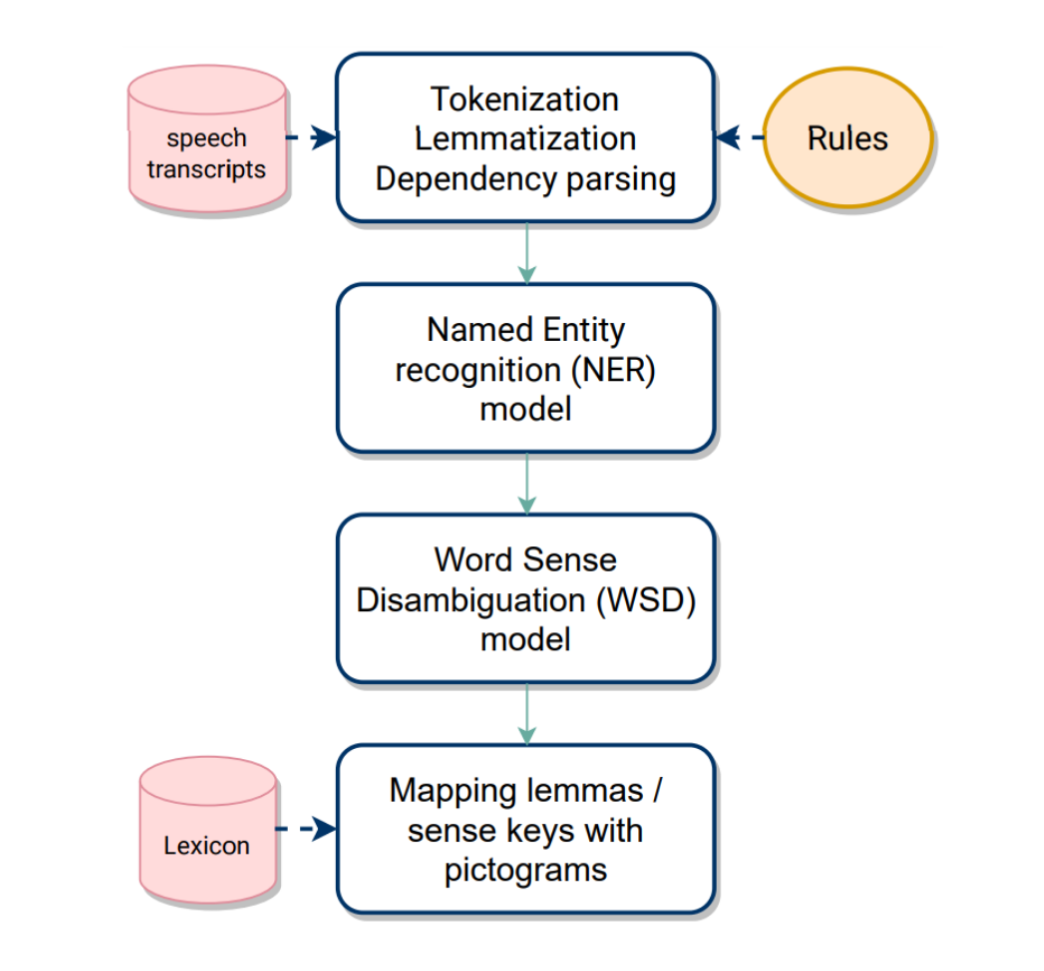
\includegraphics[width=0.45\textwidth]{img/propicto orfeo pipeline.png}
    \caption{Flujo seguido para crear los corpus Propicto, descrito para \textit{Propicto-Orfeo} \cite{macaire2024propicto}; \textit{Propicto-CommonVoice} se generó con el mismo formalismo de reglas. Las oraciones de ejemplo representadas en pictogramas se obtuvieron mediante traducción automática.}
    \label{fig:propicto_pipeline}
\end{figure}
% VERIFICAR: en el documento se usan dos keys distintas, macaire2024 y macaire2024propicto. Unificar.

Esta característica tiene una consecuencia directa: si un modelo solo aprende la relación entre un texto y su secuencia de pictogramas, y esa secuencia se obtuvo con reglas fijas, su desempeño queda limitado por esas mismas reglas. Lo ideal sería que el modelo aprendiera un idioma nuevo: el de los pictogramas o, en su defecto, el de sus identificadores.

\subsection{Alternativa explorada: xP3mt}
Para enseñar un idioma nuevo a un modelo de lenguaje se revisó el trabajo ConlangBench \citep{jeong_conlangbench_2026}, en el que se ajustan modelos de lenguaje con LoRA para traducir, en ambas direcciones, entre el inglés y lenguas ficticias como el élfico. Sus resultados muestran que los modelos se apoyan en el conocimiento de los idiomas naturales que adquirieron durante el preentrenamiento. A partir de esta idea se exploró ir más allá de la traducción: entrenar con instrucciones variadas (resumir, ampliar textos, responder preguntas, clasificar o predecir), de modo que el modelo usara el nuevo lenguaje desde distintos enfoques en lugar de memorizar una correspondencia. Este planteamiento se inspira en el ajuste multitarea, que mejora la capacidad de los modelos para generalizar a tareas e idiomas nuevos \cite{muennighoff2022crosslingual}.

Con esta idea se consideró el conjunto de datos xP3mt \cite{muennighoff2022crosslingual}, creado por BigScience. Es una variante de xP3 (\textit{Crosslingual Public Pool of Prompts}), una colección de tareas de PLN (preguntas y respuestas, resumen, inferencia, paráfrasis, traducción, entre otras) en formato instrucción--respuesta, en 46 idiomas. En xP3mt las instrucciones se tradujeron automáticamente al idioma de cada ejemplo. El conjunto está disponible en Hugging Face (\texttt{bigscience/xP3mt}); la configuración en español tiene alrededor de 3.37 millones de registros con dos campos: \texttt{inputs} y \texttt{targets}.

La propuesta era aplicar las reglas de \textit{Propicto} solo a la columna \texttt{targets}. Así el modelo aprendería a responder instrucciones con secuencias de pictogramas.

Las pruebas con xP3mt orientaron la elección hacia un corpus diseñado específicamente para pictogramas. Las salidas de xP3mt son largas y complejas, como muestra la Tabla~\ref{tab:ejemplos_xp3mt}, y muchas de sus palabras no tienen un pictograma equivalente en ARASAAC, por lo que aprovecharlo requeriría validar manualmente cada traducción. Por ello se optó por un corpus cuyas secuencias ya están asociadas a pictogramas, como se describe a continuación.

\begin{table}[htbp]
    \centering
    \small
    \caption{Ejemplos del subconjunto en español de xP3mt. Los textos largos se recortaron con [\dots].}
    \label{tab:ejemplos_xp3mt}
    \begin{tabularx}{\textwidth}{>{\raggedright\arraybackslash}X >{\raggedright\arraybackslash}X}
        \toprule
        \textbf{inputs} & \textbf{targets} \\
        \midrule
        Crea la carpeta que quieras sincronizar, si es necesario. Abre el menú Inicio. Abre el Explorador de archivos. [\dots] I'm interested in that, but I only have a few mins. Can you give me at most the first 500 characters of a detailed explanation in Spanish about that?
        & Si quieres sincronizar una nueva carpeta en vez de hacerlo con una que ya existe, crea la carpeta siguiendo estos pasos: Ve a la ubicación donde quieras crear la carpeta (por ejemplo, el Escritorio). Haz clic derecho en un espacio en blanco. Selecciona Nuevo. [\dots] \\
        \midrule
        Mu mutima gw'olunaku, abatambuze balaba ebifaanani ebyamazzi nga balowooza nti mazzi (oba ebintu ebirala). The previous text is in Ganda. Here is a translation to Spanish:
        & Durante el calor diurno, es posible que los turistas vean espejismos que generan la ilusión de visualizar agua, entre otros. \\
        \midrule
        {}[Texto en hindi con instrucciones para obtener un recibo de Uber] Write a summary of the previous text in Spanish:
        & Ve a https://riders.uber.com en un navegador web. Inicia sesión en Uber. Haz clic en Mis viajes. Selecciona un viaje. Haz clic en Reenviar. \\
        \bottomrule
    \end{tabularx}
\end{table}

\subsection{Conjunto de datos elegido: Propicto-CommonVoice}
La familia de corpus Propicto incluye dos conjuntos en francés construidos con el mismo formalismo de reglas y el mismo vocabulario de ARASAAC \cite{macaire2024, propicto_commonvoice}. \textit{Propicto-Orfeo} contiene cerca de 290 mil enunciados de habla espontánea, es decir, conversaciones reales transcritas. \textit{Propicto-CommonVoice}, construido a partir de la versión 15.0 del corpus Common Voice en francés, contiene cerca de 560 mil enunciados de habla leída: personas que leen en voz alta oraciones escritas \cite{propicto_commonvoice}.

Se decidió usar \textit{Propicto-CommonVoice} por dos razones. Primero, es casi el doble de grande: su partición de entrenamiento tiene 527,554 registros, frente a 231,374 de \textit{Propicto-Orfeo}. Segundo, sus oraciones están escritas y bien formadas, sin titubeos ni repeticiones, por lo que se parecen más a la entrada que recibirá el modelo, ya que el usuario escribe el texto que desea traducir. El corpus mantiene sus particiones originales de entrenamiento, validación y prueba (527,554, 16,132 y 16,132 registros). Cada registro tiene cuatro campos: el identificador del audio (\texttt{clips}), el texto fuente (\texttt{text}), la lista de identificadores de pictograma (\texttt{pictos}) y las palabras clave en francés asociadas a cada pictograma (\texttt{tokens}). En este trabajo se usan \texttt{text} y \texttt{pictos}.

El corpus está en francés; para que el modelo funcione en varios idiomas, el texto fuente se traducirá a otros cinco. Este proceso se describe en la fase de ingeniería de datos (Sección~\ref{sec:seleccion_idiomas}).

\subsection{Vocabulario de pictogramas: API de ARASAAC}
\label{sec:api_arasaac}

El sistema necesita consultar el catálogo de ARASAAC en tres momentos: (i)~al construir el conjunto de datos, para asociar términos con pictogramas; (ii)~después de la inferencia, para convertir los términos generados por el modelo en identificadores; y (iii)~en la interfaz web, para mostrar las imágenes. Para esto se usa directamente la API REST pública de ARASAAC (\url{https://api.arasaac.org/v1}), sin construir una copia local del catálogo. La Tabla~\ref{tab:api_arasaac} resume los puntos de acceso que se usan.

\begin{table}[H]
\centering
\caption{Puntos de acceso de la API de ARASAAC utilizados en el proyecto.}
\label{tab:api_arasaac}
\small
\renewcommand{\arraystretch}{1.25}
\begin{tabularx}{\linewidth}{@{}
  >{\raggedright\arraybackslash}p{0.38\linewidth}
  >{\raggedright\arraybackslash}X
  >{\raggedright\arraybackslash}X@{}}
\toprule
\textbf{Endpoint} & \textbf{Descripción} & \textbf{Uso} \\
\midrule
\texttt{\footnotesize GET /pictograms/\allowbreak\{idioma\}/\allowbreak search/\allowbreak\{texto\}} &
Busca pictogramas cuyas palabras clave contienen el texto &
Revisión manual de casos \\
\addlinespace
\texttt{\footnotesize GET /pictograms/\allowbreak\{idioma\}/\allowbreak\{id\}} &
Devuelve los metadatos de un pictograma, incluidas sus palabras clave &
Validación de identificadores generados y conversión de ID a término en la evaluación \\
\addlinespace
\texttt{\footnotesize GET /keywords/\allowbreak\{idioma\}} &
Lista las palabras clave disponibles en el idioma &
Análisis de cobertura del vocabulario \\
\addlinespace
\texttt{\footnotesize GET /pictograms/\allowbreak\{id\}?\allowbreak download=\allowbreak false} &
Devuelve la imagen del pictograma &
Visualización en la interfaz web \\
\addlinespace
\texttt{\footnotesize static.arasaac.org/\allowbreak pictograms/\allowbreak\{id\}/\allowbreak\{id\}\_500.png} &
Imagen PNG estática (500~px) servida desde el CDN &
Visualización en la interfaz web \\
\bottomrule
\end{tabularx}
\end{table}

\subsubsection{Estructura de la respuesta}
Cada pictograma se devuelve como un objeto JSON. Los campos útiles para este trabajo son: \texttt{\_id} (el identificador numérico, el mismo de la columna \texttt{pictos}), \texttt{keywords} (lista de objetos con \texttt{keyword}, \texttt{type}, \texttt{meaning} y \texttt{plural}), \texttt{categories}, \texttt{tags} y \texttt{synsets} (enlaces a WordNet). Los campos \texttt{schematic}, \texttt{violence} y \texttt{sex} permiten filtrar pictogramas inadecuados o no esquemáticos.
\subsubsection{Ejemplo de consulta}
El Código~\ref{lst:api_arasaac} muestra cómo se comprueba que un identificador existe, se lee su palabra clave y se obtiene la URL de su imagen.

\begin{lstlisting}[
  language=Python,
  basicstyle=\ttfamily\small,
  breaklines=true,
  frame=single,
  caption={Consulta a la API de ARASAAC en Python.},
  label={lst:api_arasaac},
  float=htbp
]
import requests

BASE = "https://api.arasaac.org/v1"
STATIC = "https://static.arasaac.org/pictograms"

# Validacion de un identificador y lectura de su palabra clave
id_picto = 2345  # ejemplo
r = requests.get(f"{BASE}/pictograms/es/{id_picto}", timeout=10)
existe = r.status_code == 200
if existe:
    palabra = r.json()["keywords"][0]["keyword"]

# URL de la imagen
url = f"{STATIC}/{id_picto}/{id_picto}_500.png"
\end{lstlisting}
\subsubsection{Licencia}
Los pictogramas son propiedad del Gobierno de Aragón, su autor es Sergio Palao y se distribuyen bajo licencia CC BY-NC-SA~\cite{arasaac}. Por ello, el uso en este trabajo es no comercial y las imágenes de la interfaz deben conservar la atribución.

%%%%%%%%%%%%%%%%%%%%%%%%%%%%%%%%%%%%%%%%%%%%%%%%%%%%%%%%%%%%%%%%%%%%%%%%%%%%%%%
\clearpage
\section{Ingeniería de datos}
\label{sec:ingenieria-datos}
%%%%%%%%%%%%%%%%%%%%%%%%%%%%%%%%%%%%%%%%%%%%%%%%%%%%%%%%%%%%%%%%%%%%%%%%%%%%%%%

En este capítulo se describe cómo se construye el corpus con el que se entrenará el modelo a partir de \textit{Propicto-CommonVoice}. Primero se explica la selección de los idiomas a los que se traduce el corpus, que combina resultados publicados con una prueba piloto propia. Después se presenta el procesamiento bidireccional de cada ejemplo y, por último, el formato final de los datos.
 
\subsection{Selección de idiomas para la traducción del corpus}
\label{sec:seleccion_idiomas}
 
El texto fuente de \textit{Propicto-CommonVoice} se traducirá a otros idiomas con NLLB-200 en su versión de 3.3B parámetros \cite{nllbteamNoLanguageLeft2022}. Los identificadores de pictograma (\texttt{pictos}) se conservan, porque no dependen del idioma. La columna \texttt{tokens} no se usa, porque sus palabras clave están en francés.
 
Traducir el corpus a muchos idiomas es costoso, y cada traducción automática introduce errores que no se pueden revisar a mano. Por eso se eligió un grupo reducido de idiomas con criterios claros y se midió la calidad de la traducción antes de aplicarla a todo el corpus.
 
\subsubsection{Criterios de preselección}
Se usaron tres criterios:
\begin{enumerate}
    \item \textbf{Calidad de la traducción de NLLB-200 desde el francés.} No tiene sentido traducir el corpus a un idioma que NLLB-200 traduce mal, porque los errores pasarían directo a los datos de entrenamiento. Para saber qué tan bien traduce NLLB-200 del francés a cada idioma se usaron resultados ya publicados, en lugar de evaluar cada idioma desde cero.
 
    Estos resultados se obtienen con FLORES-200 \cite{nllbteamNoLanguageLeft2022}, un conjunto de prueba formado por las mismas oraciones traducidas por personas a unos 200 idiomas. Como las oraciones son las mismas en todos los idiomas, sirve para comparar a un sistema de traducción en muchas direcciones. Se toma la oración en francés, NLLB-200 la traduce al idioma destino y su traducción se compara con la traducción humana mediante la métrica chrF++ (Sección~\ref{par:chrf}). Un valor de chrF++ más alto indica que la traducción automática se parece más a la humana.
 
    El grupo Helsinki-NLP publica una tabla (\textit{External MT Leaderboard}) con el chrF++ de NLLB-200 para las 202 direcciones que tienen al francés como idioma fuente. % PENDIENTE: agregar la referencia de la tabla de Helsinki-NLP en Zotero.
    Los idiomas se ordenaron de mayor a menor chrF++ y se tomaron como candidatos los 40 primeros.
 
    Este criterio tiene dos limitaciones. La primera es que FLORES-200 se compone de oraciones de Wikipedia, largas y de tema enciclopédico, distintas a las oraciones de \textit{Propicto-CommonVoice}, que suelen ser más cortas y de temas variados. La segunda es que chrF++ no es comparable entre idiomas con sistemas de escritura distintos. Por eso el chrF++ solo se usó para preseleccionar, y la calidad se midió después directamente en nuestros datos con una prueba piloto.
 
    \item \textbf{Cobertura en Qwen3}: el idioma debe estar entre los 119 del preentrenamiento de Qwen3 \cite{yang2025qwen3}. Si el modelo base apenas conoce un idioma, tendría que aprenderlo además de los pictogramas. Este filtro casi no descartó opciones: de los 40 candidatos, solo unos pocos, como el esperanto, el malgache o el zulú, quedan fuera.
    \item \textbf{Relevancia para el proyecto}: el español por el contexto de este trabajo y el inglés por ser el idioma con más presencia en el preentrenamiento de cualquier LLM.
\end{enumerate}
 
Con estos criterios se preseleccionaron ocho idiomas: español (chrF++ de 50.2), inglés (67.3), alemán (53.2), ruso (48.2), turco (46.5), vietnamita (51.2), hindi (46.4) y árabe (44.3). Se descartaron el japonés y el chino. Qwen3 los maneja bien, pero sus valores de chrF++ (19.9 y 16.7) no sirven para juzgar la traducción: la métrica penaliza las escrituras sin espacios entre palabras. Por la misma razón, chrF++ no sirve para comparar idiomas con escrituras distintas, y fue necesaria una prueba adicional.
 
\subsubsection{Prueba piloto}
Como las oraciones de FLORES-200 son distintas a las del corpus elegido, los valores de chrF++ no garantizan la calidad en nuestros datos. Para medirla directamente se tomó una muestra aleatoria de 200 oraciones de \textit{Propicto-CommonVoice}, con semilla fija, sin duplicados ni oraciones de menos de tres palabras.
Cada oración se tradujo a los ocho idiomas con NLLB-200 3.3B (búsqueda por haz de tamaño 4, precisión de 16 bits).
 
Las 1,600 traducciones se evaluaron con CometKiwi (\texttt{wmt22-cometkiwi-da}) \cite{rei2022cometkiwi}, descrita en la Sección~\ref{par:cometkiwi}. Se eligió esta métrica por dos razones. Primero, no necesita una traducción de referencia, y no existen traducciones humanas de \textit{Propicto} a estos idiomas. Segundo, a diferencia de chrF++, sus valores (de 0 a 1) sí se pueden comparar entre idiomas. Por cada idioma se calculó la media, la mediana, el percentil 10, el porcentaje de traducciones por debajo de 0.70 y un intervalo de confianza al 95\% de la media mediante \textit{bootstrap} con 1,000 remuestreos. Los resultados están en la Tabla~\ref{tab:piloto_cometkiwi}.
 
\begin{table}[H]
    \centering
    \small
    \caption{Calidad estimada con CometKiwi de la traducción con NLLB-200 3.3B de 200 oraciones de \textit{Propicto-CommonVoice}, del francés a cada idioma candidato. Se incluye el chrF++ en FLORES-200 como referencia.}
    \label{tab:piloto_cometkiwi}
    \begin{tabular}{lcccccc}
        \toprule
        \textbf{Idioma} & \textbf{chrF++} & \textbf{Media} & \textbf{IC 95\%} & \textbf{Mediana} & \textbf{P10} & \textbf{\% < 0.70} \\
        \midrule
        Inglés     & 67.3 & 0.824 & [0.815, 0.834] & 0.846 & 0.743 & 6.0 \\
        Español    & 50.2 & 0.785 & [0.767, 0.805] & 0.837 & 0.585 & 20.0 \\
        Alemán     & 53.2 & 0.781 & [0.764, 0.797] & 0.834 & 0.597 & 19.0 \\
        Turco      & 46.5 & 0.777 & [0.759, 0.796] & 0.832 & 0.605 & 24.0 \\
        Hindi      & 46.4 & 0.777 & [0.760, 0.796] & 0.832 & 0.544 & 20.5 \\
        Ruso       & 48.2 & 0.776 & [0.759, 0.795] & 0.831 & 0.583 & 23.0 \\
        Vietnamita & 51.2 & 0.761 & [0.742, 0.780] & 0.809 & 0.560 & 22.5 \\
        Árabe      & 44.3 & 0.734 & [0.712, 0.756] & 0.792 & 0.509 & 30.0 \\
        \bottomrule
    \end{tabular}
\end{table}

\subsubsection{Interpretación}
La traducción típica es buena en todos los idiomas, con medianas entre 0.79 y 0.85. El inglés es el mejor: solo el 6\% de sus traducciones queda por debajo de 0.70. Español, alemán, turco, hindi y ruso tienen medias entre 0.776 y 0.785, y sus intervalos de confianza se traslapan casi por completo. Con esta muestra no hay evidencia de que alguno se traduzca mejor que otro. El vietnamita queda un poco por debajo. El árabe es el peor: su intervalo no se traslapa con el del inglés, el 30\% de sus traducciones está por debajo de 0.70 y sus traducciones miden en mediana el 72\% de la oración original (en los demás idiomas, cerca del 90\% o más). Esto sugiere que se omite contenido.

\subsubsection{Decisión}
Se traducirá el corpus a cinco idiomas: español, inglés, alemán, ruso y turco, cuya calidad de traducción resultó equivalente. Los 527,554 registros de entrenamiento de \textit{Propicto-CommonVoice} se reparten en partes iguales entre los cinco idiomas: \textbf{unos 105,500 registros por idioma}. Así se evita el sesgo hacia una sola lengua y el corpus mantiene un tamaño manejable.

\subsubsection{Ventajas de entrenar con varios idiomas}
Entrenar un solo modelo con datos en varios idiomas tiene respaldo en la literatura. En traducción automática, Johnson et al.\ \cite{johnson2017google} mostraron que un único modelo entrenado con varios pares de idiomas a menudo mejora la calidad de todos ellos sin aumentar el número de parámetros, e incluso traduce entre pares que nunca vio durante el entrenamiento. En el ajuste de modelos de lenguaje, Muennighoff et al.\ \cite{muennighoff2022crosslingual} encontraron que ajustar con tareas en varios idiomas mejora el desempeño tanto en inglés como en los demás idiomas, y que el modelo logra generalizar incluso a idiomas que no vio de forma intencional durante el ajuste.

Dos trabajos más recientes son especialmente cercanos al diseño de este corpus. Shaham et al.\ \cite{shaham2024multilingual} reportan que los modelos ajustados con una mezcla de idiomas igualan o superan en cada idioma a los ajustados en uno solo, aun con unas diez veces menos ejemplos por idioma, y que basta con incluir de dos a cuatro idiomas para mejorar notablemente la generalización a otros. Chen et al.\ \cite{chen2024monolingual}, en un escenario similar al de este trabajo, con datos traducidos automáticamente y ajuste mediante LoRA o ajuste completo, encontraron que, con el mismo presupuesto de cómputo, un modelo multilingüe rinde al menos igual que entrenar un modelo por idioma, y que con menos datos por idioma resulta igual de eficaz y más robusto.

Con base en estos resultados, se espera que repartir el corpus entre cinco idiomas favorezca la generalización del modelo sin perjudicar su desempeño en cada idioma. Se reconoce también que mezclar demasiados idiomas en un modelo de capacidad fija puede afectar a los idiomas con más datos, un fenómeno conocido como interferencia \cite{aharoni2019massively, conneau2020unsupervised}. Limitar el corpus a cinco idiomas, todos presentes en el preentrenamiento de Qwen3, reduce este riesgo.

\subsection{Procesamiento bidireccional}
Siguiendo el procedimiento de ConlangBench \citep{jeong_conlangbench_2026}, que duplica cada ejemplo como traducción en ambos sentidos, cada muestra se usa en dos direcciones:
\begin{itemize}
    \item \textbf{Directa (texto $\rightarrow$ identificadores):} la tarea principal del sistema. Unos 105,500 ejemplos por idioma.
    \item \textbf{Inversa (identificadores $\rightarrow$ texto):} los mismos ejemplos con los papeles invertidos. Como los identificadores son códigos numéricos sin significado léxico propio, esta dirección sirve para anclar cada identificador al significado del texto en el que aparece, y ayuda al modelo a aprender la relación en ambos sentidos durante el ajuste con LoRA \citep{hu2021lora}.
\end{itemize}
Cada idioma aporta unos 211 mil ejemplos, y el corpus de entrenamiento final tiene \textbf{alrededor de 1.05 millones de registros}.

\subsection{Formato final}
Cada ejemplo del corpus tiene dos campos: el texto traducido en \texttt{src} y la lista de identificadores de pictograma en \texttt{pictos}. El modelo aprende a predecir directamente la secuencia de identificadores a partir del texto, sin generar términos intermedios. La columna \texttt{tokens} original no se usa, porque sus palabras clave están en francés y no son parte de la salida del modelo.

Por ejemplo, la oración «El niño come una manzana» corresponde a la secuencia \texttt{2345 6789 1234}, donde cada número es el identificador de ARASAAC del pictograma de «niño», «comer» y «manzana», respectivamente.
% REEMPLAZAR los IDs de ejemplo por los reales..
% PENDIENTE: confirmar en qué idioma quedan los términos de tgt (uno solo para todos los idiomas fuente, o uno por idioma) y qué regla se usa cuando un pictograma tiene varias palabras clave.

Los términos compuestos se escriben unidos por guion bajo, como \texttt{cepillarse\_dientes}. Por ejemplo, la oración «El niño come una manzana» corresponde a los términos \texttt{niño comer manzana}.


%%%%%%%%%%%%%%%%%%%%%%%%%%%%%%%%%%%%%%%%%%%%%%%%%%%%%%%%%%%%%%%%%%%%%%%%%%%%%%%
\clearpage
\section{Ingeniería del modelo de aprendizaje automático}
\label{sec:ingenieria-modelo}
%%%%%%%%%%%%%%%%%%%%%%%%%%%%%%%%%%%%%%%%%%%%%%%%%%%%%%%%%%%%%%%%%%%%%%%%%%%%%%%

En este capítulo se presenta el modelo de traducción propuesto. Se justifica la elección del modelo base, Qwen3-4B, y se describen las dos configuraciones de vocabulario que se compararán, el ajuste con LoRA (\textit{Low-Rank Adaptation}, adaptación de bajo rango), el procedimiento de entrenamiento e inferencia y la arquitectura completa del sistema. El capítulo cierra con el análisis de viabilidad de los recursos de cómputo necesarios para el entrenamiento.

\subsection{Modelo utilizado y justificación}
\label{sec:modelo}

Se usa Qwen3-4B~\cite{yang2025qwen3}, un modelo de lenguaje denso y \textit{decoder-only}. La idea del trabajo es enseñar a un modelo que ya domina varios idiomas a escribir en el <<idioma>> de los identificadores de ARASAAC, como si se le enseñara un idioma nuevo. Chinese-LLaMA sigue un planteamiento parecido: amplía el vocabulario de LLaMA y lo adapta con LoRA~\cite{cui2023efficient}.

Las razones para elegir Qwen3-4B son:
\begin{itemize}
    \item \textbf{Cobertura de idiomas.} Qwen3 se preentrenó con 36 billones de \textit{tokens} en 119 idiomas y dialectos~\cite{yang2025qwen3}, incluidos los cinco del corpus. El modelo no tiene que aprender el idioma además de los pictogramas.
    \item \textbf{Tokenizador.} Opera a nivel de bytes, por lo que puede representar cualquier cadena. Los números se dividen en dígitos individuales, así que un identificador de pictograma se representa como una secuencia corta de tokens.
    \item \textbf{Embeddings compartidos.} En los tamaños de hasta 4B (0.6B, 1.7B y 4B), Qwen3 comparte los pesos del \textit{embedding} de entrada y de la capa de salida; 4B es el mayor de ellos y el de 8B ya no los comparte~\cite{yang2025qwen3}. Esto simplifica entrenar los \textit{tokens} nuevos de la configuración~B, porque una sola actualización cubre ambas matrices~\cite{peft}.
    \item \textbf{Capacidad y costo.} LoRA aprende menos que el ajuste completo cuando debe adquirir conocimiento nuevo~\cite{biderman2024lora}, así que conviene partir del modelo más capaz que siga siendo manejable. Con unos 8~GB en 16 bits y solo las matrices $A$ y $B$ entrenables, el ajuste es viable con los recursos de la Sección~\ref{sec:viabilidad}.
    \item \textbf{Licencia.} Sus pesos se publican con licencia Apache~2.0~\cite{yang2025qwen3}.
\end{itemize}

Se prefirió Qwen3-4B sobre Qwen3.5, sucesor de esta familia, que es multimodal y combina atención con capas Gated DeltaNet~\cite{qwen35card}. Una arquitectura de solo texto se ajusta mejor a una tarea con oraciones cortas y permite atribuir con claridad las diferencias entre las configuraciones~A y~B al vocabulario.

Los sistemas de ToPicto 2026 usan modelos codificador--decodificador pequeños con ajuste completo: T5-base, FLAN-T5-base y BART-base~\cite{Sudharshan2026,GuzmanColomina2026,Gokul2026}. Sus resultados sirven como referencia para el modelo propuesto, y al compararlos se tomará en cuenta que este es de mayor tamaño.

\subsection{Vocabulario: configuraciones A y B}
Un identificador como \texttt{2345} no es una sola unidad para el tokenizador: lo divide en dígitos. Un identificador es entonces una secuencia de varios tokens, y el modelo debe aprender qué combinaciones de dígitos corresponden a cada pictograma. Los equipos de ToPicto 2026, que generan términos, resolvieron un problema parecido (términos compuestos que el tokenizador divide en varias piezas) de formas distintas:
\begin{itemize}
    \item Los dos primeros lugares no cambiaron el vocabulario~\citep{Sudharshan2026,GuzmanColomina2026}.
    \item El tercero añadió como tokens completos los términos que aparecen al menos cinco veces en los \texttt{tgt} de entrenamiento y que el tokenizador divide en más de una pieza, con embeddings iniciados al azar~\citep{Gokul2026}.
    \item Otro equipo añadió los 2,041 términos compuestos a T5-large y quedó en noveno lugar~\citep{Adithiyaa2026}, aunque su sistema también difiere en el modelo y en la decodificación.
\end{itemize}
Los tres primeros sistemas quedaron separados por menos de un punto de sacreBLEU~\citep{Hjuler2026}, así que estos resultados no indican si ampliar el vocabulario ayuda. Por eso se prueban dos configuraciones, adaptando la regla del tercer lugar a identificadores:
\begin{itemize}
    \item \textbf{Configuración A:} se conserva el vocabulario original del modelo. Cada identificador se escribe como una secuencia de dígitos.
    \item \textbf{Configuración B:} cada identificador que aparece al menos cinco veces en los \texttt{pictos} de entrenamiento se añade como un token completo (por ejemplo, \texttt{\textless picto\_2345\textgreater}). Como un identificador no tiene piezas con significado que promediar, el embedding de cada token nuevo se inicia con el promedio de los embeddings de las piezas en que el tokenizador divide la palabra clave principal del pictograma, obtenida de la API de ARASAAC. Es una variante de la inicialización por promedio de Hewitt~\citep{hewitt2021initializing}. Así el token empieza cerca del significado del pictograma en el espacio del modelo.
\end{itemize}

\subsection{Ajuste con LoRA}
LoRA~\citep{hu2021lora} congela los pesos originales $W_0 \in \mathbb{R}^{d \times k}$ y les suma una actualización de bajo rango $\Delta W = BA$, donde $A \in \mathbb{R}^{r \times k}$ se inicia con una distribución gaussiana, $B \in \mathbb{R}^{d \times r}$ se inicia en cero y $r \ll \min(d,k)$. La salida de la capa es:
\begin{equation}
h = W_0x + \frac{\alpha}{r}BAx
\end{equation}
Como $B$ empieza en cero, al inicio $\Delta W = 0$ y el modelo conserva su comportamiento original.

LoRA se aplica en cada capa del Transformer, tanto a las proyecciones de atención como a las de la red \textit{feed-forward}. Se incluyen estas últimas porque LoRA aprende menos que el ajuste completo cuando debe adquirir conocimiento nuevo~\citep{biderman2024lora}, y Chinese-LLaMA también lo aplicó a atención y MLP~\citep{cui2023efficient}.

\subsubsection{Parámetros entrenables}
En ambas configuraciones se entrenan $A$ y $B$. En la configuración B también se entrenan las filas nuevas de la matriz de embeddings y de la capa de salida (una por cada identificador añadido), con el parámetro \texttt{trainable\_token\_indices} de PEFT~\citep{peft}.

\subsection{Entrenamiento e inferencia}
Cada ejemplo se presenta como una instrucción seguida del texto y de la secuencia de identificadores. Por ejemplo: \texttt{Traduce a pictogramas: El niño come una manzana.} seguido de \texttt{2345 6789 1234}. Los equipos de ToPicto que probaron un prefijo de tarea lo conservaron~\citep{Sudharshan2026,GuzmanColomina2026}. En la dirección inversa se usa una instrucción equivalente que pide el texto a partir de los identificadores.
% REEMPLAZAR los IDs de ejemplo por los reales.

La pérdida es la entropía cruzada y se calcula solo sobre la parte de la respuesta. En inferencia se usa decodificación voraz o búsqueda por haz; el ancho del haz y la penalización de longitud se eligen con el conjunto de validación. Los tres primeros sistemas de ToPicto usaron decodificación voraz o haces de 12 y 16, según el equipo~\citep{Sudharshan2026,GuzmanColomina2026,Gokul2026}.

Al ser un modelo generativo, puede producir identificadores que no existen en ARASAAC. Cada identificador generado se comprueba con el punto de acceso \texttt{GET /pictograms/\{idioma\}/\{id\}} de la API (Sección~\ref{sec:api_arasaac}) y los inexistentes se descartan de la secuencia final.

La Figura~\ref{fig:arquitectura_lora_arasaac} resume el sistema. Primero se construye el corpus: \textit{Propicto-CommonVoice} se traduce a cinco idiomas y se procesa en dos direcciones. Después, Qwen3-4B se ajusta con LoRA en las dos configuraciones de vocabulario. Por último, en inferencia, el modelo genera directamente los identificadores de ARASAAC y se descartan los que no existen en el catálogo.

\begin{figure}[htbp]
  \centering
  \shorthandoff{<>}% evita conflictos de babel (español) con las flechas de TikZ
  \resizebox{\textwidth}{!}{%
  \begin{tikzpicture}[
    font=\sffamily,
    >=Stealth,
    box/.style={rectangle, draw=blue!70!black, fill=blue!5, thick, rounded corners=4pt, minimum height=1cm, align=center, inner sep=8pt},
    lorabox/.style={rectangle, draw=orange!80!black, fill=orange!10, thick, rounded corners=4pt, align=center, inner sep=6pt, text width=3.0cm},
    data/.style={rectangle, draw=emerald!70!black, fill=emerald!10, thick, rounded corners=8pt, align=center, inner sep=7pt, text width=4.4cm},
    loss/.style={rectangle, draw=purple!70!black, fill=purple!10, thick, rounded corners=4pt, align=center, inner sep=6pt},
    post/.style={rectangle, draw=gray!70!black, dashed, thick, fill=white, rounded corners=6pt, align=center, inner sep=7pt, text width=4.2cm},
    arrow/.style={->, thick, draw=gray!80!black},
    dasharrow/.style={->, thick, dashed, draw=orange!80!black},
    postarrow/.style={->, thick, dashed, draw=gray!70!black},
    lbl/.style={font=\small\sffamily, fill=white, inner sep=2pt},
    container/.style={draw=gray!60, dashed, inner sep=14pt, rounded corners=6pt, fill=gray!4!white}
  ]

    %%%%%%%%%%%%%%%%%%%% DATASET %%%%%%%%%%%%%%%%%%%%
    \node (corpus) [data] at (0,0) {\textbf{1. Propicto-CommonVoice}\\ 527K registros en franc\'es};
    \node (trad) [data] at (6.33,0) {\textbf{2. Traducci\'on con NLLB-200}\\ 5 idiomas, $\sim$105K c/u};
    \node (terms) [data] at (12.67,0) {\textbf{3. Identificadores}\\ se usa \texttt{pictos} como salida\\ + direcci\'on inversa ($\times 2$)};
    \node (dataset) [data, fill=emerald!20] at (19,0) {\textbf{4. Dataset final}\\ ($\approx 1.05\text{M}$ registros)\\ \textit{``El ni\~no come una manzana.''}\\ \texttt{2345 6789 1234}};

    \draw[arrow] (corpus) -- (trad);
    \draw[arrow] (trad) -- (terms);
    \draw[arrow] (terms) -- (dataset);

    %%%%%%%%%%%%%%%%%%%% FINE-TUNING %%%%%%%%%%%%%%%%%%%%
    \node (emb) [box, text width=3.4cm] at (0,-7.5) {\textbf{Embedding de entrada}\\ tokens del \texttt{src}\\ \textcolor{orange!70!black}{+ filas nuevas (configuraci\'on B)}};

    \node (w0) [box, fill=blue!15, minimum height=1.8cm, text width=4.2cm] at (9.5,-5.7) {\textbf{Pesos congelados} ($W_0$)\\ $d \times k$\\ \small(\textit{frozen weights})};

    \node (lora_A) [lorabox] at (5.6,-9.3) {\textbf{Matriz LoRA $A$}\\ $r \times k$ \small(gaussiana)};
    \node (lora_B) [lorabox] at (10.2,-9.3) {\textbf{Matriz LoRA $B$}\\ $d \times r$ \small(ceros)};
    \node (scale) [lorabox, fill=orange!25, text width=1.5cm] at (13.4,-9.3) {$\times\,\alpha/r$};

    \node (sum) [circle, draw=blue!80!black, fill=blue!20, thick, inner sep=3pt] at (15.4,-7.5) {\Large$+$};

    \coordinate (split) at (3.0,-7.5);
    \draw[thick, draw=gray!80!black] (emb.east) -- (split);
    \draw[arrow] (split) |- (w0.west);
    \draw[arrow] (split) |- (lora_A.west);

    \draw[arrow] (lora_A) -- (lora_B);
    \node[lbl] at ($(lora_A.east)!0.5!(lora_B.west)+(0,0.9)$) {$r \ll \min(d,k)$};
    \draw[arrow] (lora_B) -- (scale);
    \draw[arrow] (w0.east) -| (sum.north);
    \draw[dasharrow] (scale.east) -| (sum.south);
    \node[lbl, text=orange!70!black, align=center] at (13.4,-8.15) {entrenable\\ $\Delta W = BA$};

    \node (tok) [lorabox, dashed, text width=4.4cm] at (0,-11.9) {\textbf{Tokenizador ampliado} (solo configuraci\'on B)\\ IDs con $\geq 5$ apariciones, un token por ID};
    \draw[dasharrow] (tok.north) -- node[lbl, right=2pt] {tokens nuevos} (emb.south);

    \node (lm_head) [box, text width=4.2cm] at (20.6,-7.5) {\textbf{LM Head} (atado al embedding)\\ \textcolor{orange!70!black}{+ filas nuevas (configuraci\'on B)}};
    \node (loss_node) [loss, text width=4.2cm] at (20.6,-4.7) {\textbf{Funci\'on de p\'erdida}\\ Cross-Entropy sobre \texttt{pictos}};
    \node (output_terms) [data, text width=4.2cm] at (20.6,-10.3) {\textbf{IDs predichos}\\ \texttt{2345 6789 1234}};
    \node (mapeo) [post] at (20.6,-13.0) {\textbf{Validaci\'on (inferencia)}\\ se descartan IDs que no existen en ARASAAC};

    \draw[arrow] (sum) -- (lm_head);
    \draw[arrow] (lm_head) -- (loss_node);
    \draw[arrow] (lm_head) -- (output_terms);
    \draw[postarrow] (output_terms) -- (mapeo);

    \draw[arrow] ($(dataset.south)+(-1.6,0)$) -- ++(0,-1.1) -| node[lbl, pos=0.12, above=2pt] {entrada $x$: \texttt{src}} (emb.north);
    \draw[arrow] ($(dataset.south)+(1.6,0)$) -- node[lbl, right=3pt] {etiqueta $y$: \texttt{pictos}} (loss_node.north);

    %%%%%%%%%%%%%%%%%%%% CONTENEDORES %%%%%%%%%%%%%%%%%%%%
    \begin{scope}[on background layer]
      \node[container, draw=emerald!60!black, fill=emerald!4!white, fit=(corpus) (trad) (terms) (dataset),
            label={[font=\bfseries\sffamily, text=emerald!80!black]above:Dataset (se construye una sola vez, antes de entrenar)}] (phaseA) {};

      \node[container, draw=blue!50!black, fill=blue!3!white, inner sep=18pt, fit=(emb) (w0) (lora_A) (sum) (lm_head) (loss_node) (output_terms) (mapeo) (tok),
            label={[font=\bfseries\sffamily, text=blue!80!black]above:Fine-tuning (en cada paso)}] (phaseB) {};

      \node[container, draw=orange!70!black, fill=orange!4!white, fit=(w0) (lora_A) (lora_B) (scale) (sum),
            label={[font=\bfseries\sffamily, text=orange!70!black, align=center]below:LLM decoder-only (Qwen3-4B) con LoRA en cada capa\\ $h = W_0x + \frac{\alpha}{r}\,BAx$}] (lora_container) {};
    \end{scope}

    %%%%%%%%%%%%%%%%%%%% LEYENDA %%%%%%%%%%%%%%%%%%%%
    \node[draw=blue!70!black, fill=blue!15, thick, minimum size=4mm] (lg1) at (-2.5,-16.2) {};
    \node[right=2mm of lg1, anchor=west] {Modelo base (pesos congelados)};
    \node[draw=orange!80!black, fill=orange!25, thick, minimum size=4mm] (lg2) at (8.5,-16.2) {};
    \node[right=2mm of lg2, anchor=west] {Par\'ametros entrenables: $A$, $B$ y, en la configuraci\'on B, las filas nuevas del vocabulario};
    \node[draw=gray!70!black, dashed, thick, fill=white, minimum size=4mm] (lg3) at (-2.5,-17.0) {};
    \node[right=2mm of lg3, anchor=west] {Validaci\'on determinista (sin entrenamiento)};

  \end{tikzpicture}
  }
  \caption{Arquitectura del sistema. El corpus \textit{Propicto-CommonVoice} se traduce a cinco idiomas y se procesa en dos direcciones ($\approx 1.05\text{M}$ registros). Qwen3-4B se ajusta con LoRA en dos configuraciones de vocabulario (A y B) para predecir directamente los identificadores de ARASAAC. En inferencia se descartan los identificadores inexistentes.}
  \label{fig:arquitectura_lora_arasaac}
\end{figure}

\subsection{Análisis de viabilidad}
\label{sec:viabilidad}

Para entrenar se necesita una GPU con memoria suficiente para Qwen3-4B en 16 bits (unos 8~GB de pesos) más las activaciones y los parámetros de LoRA. La Tabla~\ref{tab:cloud-services} compara los servicios de cómputo en la nube revisados.
\clearpage
% PENDIENTE: indicar qué servicio se eligió y una estimación de horas de GPU para ~1.05M registros.

\begin{table}[H]
\centering
\caption{Comparación de servicios de cómputo en la nube para el ajuste del modelo.}
\label{tab:cloud-services}
\small
\begin{tabularx}{\textwidth}{@{}X X X X X@{}}
\toprule
\textbf{Servicio} & \textbf{Nivel gratuito} & \textbf{Límite de sesión} & \textbf{Acceso root/SSH} & \textbf{Costo GPU dedicada} \\
\midrule
Kaggle Notebooks       & 30 h GPU/semana (T4/P100) & 9--12 h/sesión & No & N/A (solo gratis) \\
Google Colab (Pro/Pro+)& Sí, T4 limitado           & 12--24 h/sesión & No & \$9.99--\$49.99/mes + créditos \\
Lightning AI Studio    & 15 créditos/mes (\textasciitilde22 h T4) & Reinicio cada 4 h & Sí (tiers pagos) & Variable por tier \\
Paperspace Gradient    & Sí (GPUs M4000/P4000)     & 6--12 h (auto-apagado) & Limitado & Desde \$0.51/h \\
RunPod                 & No                        & Sin límite & Sí & Desde \$0.17/h \\
Vast.ai                & No                        & Sin límite (según host) & Sí & Desde \$0.07/h \\
Lambda Labs            & No                        & Sin límite & Sí & Variable, on-demand/reservado \\
Hugging Face Jobs      & No                        & Por trabajo & N/A (contenedor) & Según hardware elegido \\
\bottomrule
\end{tabularx}
\end{table}

%%%%%%%%%%%%%%%%%%%%%%%%%%%%%%%%%%%%%%%%%%%%%%%%%%%%%%%%%%%%%%%%%%%%%%%%%%%%%%%
\clearpage
\section{Evaluación de los modelos}
\label{sec:evaluacion}
%%%%%%%%%%%%%%%%%%%%%%%%%%%%%%%%%%%%%%%%%%%%%%%%%%%%%%%%%%%%%%%%%%%%%%%%%%%%%%%

En este capítulo se define cómo se medirá el desempeño del modelo de traducción: qué métricas se usarán, sobre qué tipo de secuencias se calcularán y qué comparaciones permitirán valorar los resultados.

Se usarán las métricas oficiales de ToPicto: sacreBLEU, METEOR y la tasa de error de términos de pictograma (PictoER)~\citep{Hjuler2026}. Como el modelo predice identificadores, las métricas se calculan principalmente sobre las secuencias de identificadores (\texttt{pictos}), donde cada identificador cuenta como una unidad.

Los sistemas de ToPicto producen términos y se evalúan sobre términos. Para compararse con ellos, los identificadores generados y los de referencia se convertirán a términos con las palabras clave de la API de ARASAAC, solo para el cálculo de la métrica. Se informará explícitamente qué resultados se calcularon sobre identificadores y cuáles sobre términos convertidos.
% PENDIENTE: definir la regla de conversión ID -> término (idioma y palabra clave) y verificar que sea la misma que usa la referencia de ToPicto.

Los identificadores generados que no existen en ARASAAC se descartan de la secuencia antes de calcular las métricas, y se registra su porcentaje.

Se harán tres comparaciones, todas con las mismas métricas y el mismo conjunto de validación:
\begin{itemize}
    \item Configuración A frente a configuración B, para medir el efecto de ampliar el vocabulario.
    \item Ambas configuraciones frente al traductor basado en reglas, que funciona como línea base.
    \item Resultados frente a los sistemas de ToPicto 2026 (Tabla~\ref{tab:sota-text-to-picto}), tomando en cuenta la diferencia de tamaño entre modelos y la conversión de identificadores a términos.
\end{itemize}

\subsection{Conjunto de prueba con anotación humana}
De manera complementaria, se contempla construir un conjunto de prueba en español anotado por personas. Las referencias de \textit{Propicto-CommonVoice} se generaron con una gramática basada en reglas \cite{macaire2024}, por lo que las métricas descritas miden qué tan bien el modelo reproduce esas reglas. Un conjunto anotado por personas permitiría comparar además las salidas del modelo con las secuencias que una persona elegiría para expresar la misma oración.

Para construirlo, participantes voluntarios seleccionarán, mediante una herramienta web sencilla con buscador y categorías de pictogramas de ARASAAC, la secuencia que mejor exprese cada oración. Las oraciones se tomarán del conjunto de prueba de \textit{Propicto-CommonVoice} traducido al español, de modo que cada una cuente con dos referencias: la generada por reglas y la elegida por personas. Cada oración será anotada por más de una persona, lo que permitirá medir el grado de acuerdo entre anotadores, y la tarea se apoyará en una guía breve que unifique criterios, por ejemplo, cómo representar el tiempo verbal o qué hacer cuando no existe un pictograma adecuado.

La evaluación principal del modelo no depende de este conjunto y se realizará con las referencias de \textit{Propicto-CommonVoice}. El conjunto con anotación humana se usará únicamente como evaluación complementaria, en la medida en que se complete.
%%%%%%%%%%%%%%%%%%%%%%%%%%%%%%%%%%%%%%%%%%%%%%%%%%%%%%%%%%%%%%%%%%%%%%%%%%%%%%%
\clearpage
\section{Despliegue}
\label{sec:despliegue}
%%%%%%%%%%%%%%%%%%%%%%%%%%%%%%%%%%%%%%%%%%%%%%%%%%%%%%%%%%%%%%%%%%%%%%%%%%%%%%%

En este capítulo se describe cómo el modelo entrenado se pondrá a disposición de las personas usuarias. El modelo se encapsulará en una API REST (\textit{Representational State Transfer}) que recibe texto en cualquiera de los cinco idiomas del corpus y devuelve la secuencia de identificadores de ARASAAC. Sobre esta API se construirá una interfaz web en la que el usuario escribe un texto y visualiza de inmediato la secuencia de pictogramas. El modelo genera directamente los identificadores, la API conserva solo los que existen en el catálogo de ARASAAC y las imágenes se cargan desde su CDN (\textit{Content Delivery Network}, red de distribución de contenidos; Tabla~\ref{tab:api_arasaac}), con la atribución que exige la licencia. El servicio se empaquetará en contenedores para que pueda desplegarse de forma reproducible en distintos entornos.
%%%%%%%%%%%%%%%%%%%%%%%%%%%%%%%%%%%%%%%%%%%%%%%%%%%%%%%%%%%%%%%%%%%%%%%%%%%%%%%
\clearpage
\section{Monitoreo y mantenimiento}
\label{sec:monitoreo}
%%%%%%%%%%%%%%%%%%%%%%%%%%%%%%%%%%%%%%%%%%%%%%%%%%%%%%%%%%%%%%%%%%%%%%%%%%%%%%%

En este capítulo se describen las acciones para asegurar que el modelo desplegado mantenga su calidad con el tiempo. Como el modelo aprende identificadores fijos del catálogo, cualquier pictograma que ARASAAC elimine, reemplace o cambie de significado se reflejaría directamente en las salidas. Por ello, el plan de monitoreo da seguimiento a tres indicadores: la disponibilidad de la API de ARASAAC, los cambios en el catálogo y el porcentaje de identificadores generados que no existen en él. Cuando alguno de estos indicadores muestre una degradación, se realizará el mantenimiento correspondiente, por ejemplo, actualizar la lista de identificadores válidos o reajustar el modelo con el catálogo vigente.

\include{Cap4}
\section{Discusión preliminar}
\label{sec:discusion}

En este capítulo se discuten los resultados obtenidos hasta esta etapa del trabajo terminal y su relación con el objetivo general. Se analizan los hallazgos de la revisión del estado del arte, las decisiones tomadas sobre los datos a partir de la prueba piloto, el diseño del modelo de traducción y los pasos que guiarán la siguiente etapa del proyecto.

\subsection{Hallazgos de la revisión del estado del arte}

La revisión del estado del arte muestra que la traducción de texto a pictogramas pasó de sistemas basados en reglas y recursos léxicos a modelos neuronales entrenados con corpus alineados. En la edición 2026 de ImageCLEFtoPicto, los sistemas mejor evaluados ajustaron modelos codificador-decodificador de las familias T5 y BART y obtuvieron valores de sacreBLEU muy cercanos entre sí, entre 51.33 y 52.55 \cite{Hjuler2026}. Esta concentración de resultados indica que variar el modelo preentrenado o sus hiperparámetros ya aporta poco, y orienta este trabajo hacia dos aspectos menos explorados: la forma en que el modelo representa los pictogramas y la cobertura de varios idiomas de entrada.

La revisión también muestra que las referencias de los corpus disponibles se generaron con una gramática basada en reglas \cite{macaire2024}. Esto se tendrá presente al interpretar las métricas automáticas, que miden qué tan cerca está una salida de esas referencias. Por ello, además de las métricas oficiales, el análisis de resultados incluirá una revisión cualitativa de ejemplos representativos.

\subsection{Decisiones sobre los datos}

El análisis de los conjuntos de datos llevó a elegir \textit{Propicto-CommonVoice} como base del corpus, por estar diseñado específicamente para la traducción a pictogramas, contar con más de 527 mil registros de entrenamiento y estar formado por oraciones escritas, cercanas al texto que escribirán las personas usuarias. Para que el modelo funcione en varios idiomas, se definió un procedimiento de traducción con NLLB-200 respaldado por evidencia: los resultados publicados en FLORES-200 permitieron preseleccionar ocho idiomas, y la prueba piloto con CometKiwi midió la calidad de la traducción directamente sobre oraciones del dominio. Las medianas de calidad estimada se ubicaron entre 0.79 y 0.85, y el español, el inglés, el alemán, el ruso y el turco mostraron una calidad equivalente, por lo que se eligieron como los cinco idiomas del corpus. Con el procesamiento bidireccional, el corpus de entrenamiento final contará con alrededor de 1.05 millones de registros distribuidos de forma equilibrada entre los cinco idiomas.

\subsection{Diseño del modelo de traducción}

El modelo propuesto ajusta Qwen3-4B con LoRA para que genere directamente los identificadores de ARASAAC, tratados como un idioma nuevo. Este diseño tiene dos ventajas frente a los sistemas de referencia. Primero, al generar identificadores, la salida corresponde de forma inequívoca a pictogramas del catálogo y puede validarse automáticamente con la API de ARASAAC. Segundo, la comparación entre las configuraciones de vocabulario A y B permitirá medir de forma controlada si representar cada identificador como un token completo mejora la traducción, una pregunta que los resultados de ImageCLEFtoPicto 2026 dejan abierta.

\subsection{Trabajo siguiente}

La siguiente etapa del proyecto se centrará en construir el corpus completo en los cinco idiomas, entrenar el modelo en sus dos configuraciones de vocabulario y evaluarlo con sacreBLEU, METEOR y PictoER frente a la línea base basada en reglas y a los sistemas de ImageCLEFtoPicto 2026. Para que esta última comparación sea válida, se definirá la regla de conversión de identificadores a términos y se reportará por separado qué resultados se calcularon sobre identificadores y cuáles sobre términos. Finalmente, el modelo con mejor desempeño se integrará en la API y en la interfaz web descritas en el capítulo~\ref{sec:despliegue}, de modo que las personas usuarias puedan escribir un texto y obtener de inmediato su secuencia de pictogramas.

Como actividad complementaria, se contempla construir un conjunto de prueba en español anotado por personas, del orden de cientos de oraciones, en el que participantes voluntarios elijan mediante una herramienta web la secuencia de pictogramas que mejor exprese cada oración (Sección~\ref{sec:evaluacion}). Este conjunto permitiría atender la limitación identificada en el estado del arte, pues las salidas del modelo podrían compararse con referencias humanas y no solo con las generadas por reglas; además, el grado de acuerdo entre anotadores ofrecería una medida de qué tan variable es la tarea para las propias personas. Su realización no condiciona el cumplimiento de los objetivos: la evaluación principal se mantiene sobre las referencias de \textit{Propicto-Orfeo}.

\section{Experimental details}
\subsection{Family 1}
\subsection{Family 2}
%again edit as necessary and add \subsubsections or \paragraphs as you wish

\bibliography{bib_tt1}

% Anexos
% \begin{appendices}
% \section*{Appendices}
\phantomsection
\addcontentsline{toc}{section}{Appendices}
Lorem ipsum dolor sit amet, consectetur adipiscing elit, sed do eiusmod tempor incididunt ut labore et dolore magna aliqua. Ut enim ad minim veniam, quis nostrud exercitation ullamco laboris nisi ut aliquip ex ea commodo consequat. Duis aute irure dolor in reprehenderit in voluptate velit esse cillum dolore eu fugiat nulla pariatur. Excepteur sint occaecat cupidatat non proident, sunt in culpa qui officia deserunt mollit anim id est laborum.
% \end{appendices}

\end{document}
